% # -*- coding: utf-8 -*-
\input{ctex4xetex.cfg}
\documentclass{ctexbook}
\usepackage[inline]{asymptote}
\usepackage{animate}
\usepackage{geometry}
\geometry{left=2.5cm,right=2.5cm,top=3.5cm,bottom=2.5cm}

% 方正系列字体设置
\setCJKmainfont[BoldFont={FZXiaoBiaoSong-B05}, ItalicFont={FZKai-Z03}]{FZShuSong_GB18030-Z01} % 书宋、小标宋、楷体
\setCJKsansfont[BoldFont={FZHei-B01}]{FZXiHei I-Z08} % 细黑、黑体
\setCJKmonofont{FZFangSong-Z02} % 仿宋

\setCJKfamilyfont{rm}[BoldFont={FZXiaoBiaoSong-B05}, ItalicFont={FZKai-Z03}]{FZShuSong_GB18030-Z01} % 同 main
\setCJKfamilyfont{sf}[BoldFont={FZHei-B01}]{FZXiHei I-Z08} % 同 sans
\setCJKfamilyfont{tt}{FZFangSong-Z02} % 同 mono

\setCJKfamilyfont{song}[BoldFont={FZXiaoBiaoSong-B05}]{FZShuSong_GB18030-Z01} % 书宋和小标宋(除无楷体外同 main)
\setCJKfamilyfont{kai}{FZKai-Z03} % 楷体
\setCJKfamilyfont{hei}[BoldFont={FZHei-B01}]{FZXiHei I-Z08} % 细黑、黑体(同 sans)
\setCJKfamilyfont{fs}{FZFangSong-Z02} % 仿宋(同 mono)

\setCJKfamilyfont{you}[BoldFont={FZZhunYuan-M02}]{FZXiYuan-M01} % 细圆、准圆
\setCJKfamilyfont{li}[ItalicFont={FZLiShu II-S06}]{FZLiShu-S01} % 隶书、隶二(italic)

\def\heiti{\CJKfamily{hei}\bfseries}



\usepackage{mflogo}

% 数学相关设置
\usepackage{amsmath}
\usepackage{amssymb}
\usepackage{bm}
\usepackage{upgreek}
\let\leq\leqslant
\let\geq\geqslant
\newcommand\set[1]{\left\{ #1 \right\}}
\newcommand\Set[2]{\left\{\, #1 \, \middle\vert \, #2 \,\right\}}
\newcommand\dif{\mathrm{d}}
\newcommand\diff{\,\dif}
\newcommand\mi{\mathrm{i}}

\usepackage{longtable}

% # -*- coding: utf-8 -*-
% 2010-07-15

\usepackage[hyperref]{xcolor}
\definecolor{bg-color}{rgb}{0.96,1,0.95}
\definecolor{shadecolor}{rgb}{0.96,1,0.95}
\definecolor{txt-color}{HTML}{000000}
\definecolor{builtin}{HTML}{DA70D6}
\definecolor{comment}{HTML}{B22222}
\definecolor{comment-delimiter}{HTML}{B22222}
\definecolor{constant}{HTML}{5F9EA0}
\definecolor{function-name}{HTML}{0000FF}
\definecolor{keyword}{HTML}{a020F0}
\definecolor{string}{HTML}{BC8F8F}
\definecolor{type}{HTML}{228B22}
\definecolor{variable-name}{HTML}{B8860B}
\definecolor{brick}{HTML}{7B0C00}

% keywords 对应 asy-keyword-name
% keywords=[2] 对应 asy-type-name
% keywords=[3] 对应 asy-function-name
% keywords=[4] 对应 asy-variable-name
\usepackage{listings}
% 语言定义
\lstdefinelanguage{Asymptote}{alsoletter={},
sensitive=true,% 大小写
keywords={and,controls,tension,atleast,curl,if,else,while,for,do,return,break,continue,struct,typedef,new,access,import,unravel,from,include,quote,static,public,private,restricted,this,explicit,true,false,null,cycle,newframe,operator},
keywords=[2]{Braid,FitResult,Label,Legend,Segment,Solution,TreeNode,abscissa,arc,arrowhead,binarytree,binarytreeNode,block,bool,bool3,bounds,bqe,circle,conic,coord,coordsys,cputime,ellipse,file,filltype,frame,grid3,guide,horner,hsv,hyperbola,indexedTransform,int,inversion,key,light,line,linefit,marginT,marker,mass,object,pair,parabola,path,path3,pen,picture,point,position,projection,real,revolution,scaleT,scientific,segment,side,slice,solution,splitface,string,surface,tensionSpecifier,ticklocate,ticksgridT,tickvalues,transform,transformation,tree,triangle,trilinear,triple,vector,vertex,void},
keywords=[3]{AND,Arc,ArcArrow,ArcArrows,Arrow,Arrows,Automatic,AvantGarde,BBox,BWRainbow,BWRainbow2,Bar,Bars,BeginArcArrow,BeginArrow,BeginBar,BeginDotMargin,BeginMargin,BeginPenMargin,Blank,Bookman,Bottom,BottomTop,Bounds,Break,Broken,BrokenLog,CLZ,CTZ,Ceil,Circle,CircleBarIntervalMarker,Cos,Courier,CrossIntervalMarker,DefaultFormat,DefaultLogFormat,Degrees,Dir,DotMargin,DotMargins,Dotted,Draw,Drawline,Embed,EndArcArrow,EndArrow,EndBar,EndDotMargin,EndMargin,EndPenMargin,Fill,FillDraw,Floor,Format,Full,Gaussian,Gaussrand,Gaussrandpair,Gradient,Grayscale,Helvetica,Hermite,HookHead,InOutTicks,InTicks,Jn,Label,Landscape,Left,LeftRight,LeftTicks,Legend,Linear,Link,Log,LogFormat,Margin,Margins,Mark,MidArcArrow,MidArrow,NOT,NewCenturySchoolBook,NoBox,NoMargin,NoModifier,NoTicks,NoTicks3,NoZero,NoZeroFormat,None,OR,OmitFormat,OmitTick,OmitTickInterval,OmitTickIntervals,OutTicks,Ox,Oy,Palatino,PaletteTicks,Pen,PenMargin,PenMargins,Pentype,Portrait,RadialShade,RadialShadeDraw,Rainbow,Range,Relative,Right,RightTicks,Rotate,Round,SQR,Scale,ScaleX,ScaleY,ScaleZ,Seascape,Segment,Shift,Sin,Slant,Spline,StickIntervalMarker,Straight,Symbol,Tan,TeXify,Ticks,Ticks3,TildeIntervalMarker,TimesRoman,Top,TrueMargin,UnFill,UpsideDown,Wheel,X,XEquals,XOR,XY,XYEquals,XYZero,XYgrid,XZEquals,XZZero,XZero,XZgrid,Y,YEquals,YXgrid,YZ,YZEquals,YZZero,YZero,YZgrid,Yn,Z,ZX,ZXgrid,ZYgrid,ZapfChancery,ZapfDingbats,_begingroup3,_cputime,_draw,_eval,_image,_labelpath,_projection,_strokepath,_texpath,aCos,aSin,aTan,abort,abs,accel,acos,acosh,acot,acsc,activatequote,add,addArrow,addMargins,addSaveFunction,addnode,addnodes,addpenarc,addpenline,adjust,alias,align,all,altitude,angabscissa,angle,angpoint,animate,annotate,anticomplementary,antipedal,apply,approximate,arc,arcarrowsize,arccircle,arcdir,arcfromcenter,arcfromfocus,arclength,arcnodesnumber,arcpoint,arcsubtended,arcsubtendedcenter,arctime,arctopath,array,arrow,arrow2,arrowbase,arrowbasepoints,arrowsize,asec,asin,asinh,ask,assert,asy,asycode,asydir,asyfigure,asyfilecode,asyinclude,asywrite,atan,atan2,atanh,atbreakpoint,atexit,atime,attach,attract,atupdate,autoformat,autoscale,autoscale3,axes,axes3,axialshade,axis,axiscoverage,azimuth,babel,background,bangles,bar,barmarksize,barsize,basealign,baseline,bbox,beep,begin,beginclip,begingroup,beginpoint,between,bevel,bezier,bezierP,bezierPP,bezierPPP,bezulate,bibliography,bibliographystyle,binarytree,binarytreeNode,binomial,binput,bins,bisector,bisectorpoint,bispline,blend,blockconnector,boutput,box,bqe,breakpoint,breakpoints,brick,buildRestoreDefaults,buildRestoreThunk,buildcycle,bulletcolor,byte,canonical,canonicalcartesiansystem,cartesiansystem,case1,case2,case3,case4,cbrt,cd,ceil,center,centerToFocus,centroid,cevian,change2,changecoordsys,checkSegment,checkconditionlength,checker,checkincreasing,checklengths,checkposition,checktriangle,choose,circle,circlebarframe,circlemarkradius,circlenodesnumber,circumcenter,circumcircle,clamped,clear,clip,clipdraw,close,cmyk,code,colatitude,collect,collinear,color,colorless,colors,colorspace,comma,compassmark,complement,complementary,concat,concurrent,cone,conic,conicnodesnumber,conictype,conj,connect,connected,connectedindex,containmentTree,contains,contour,contour3,contouredges,controlSpecifier,convert,coordinates,coordsys,copy,cos,cosh,cot,countIntersections,cputime,crop,cropcode,cross,crossframe,crosshatch,crossmarksize,csc,cubicroots,curabscissa,curlSpecifier,curpoint,currentarrow,currentexitfunction,currentmomarrow,currentpolarconicroutine,curve,cut,cutafter,cutbefore,cyclic,cylinder,deactivatequote,debugger,deconstruct,defaultdir,defaultformat,defaultpen,defined,degenerate,degrees,delete,deletepreamble,determinant,diagonal,diamond,diffdiv,dir,dirSpecifier,dirtime,display,distance,divisors,do_overpaint,dot,dotframe,dotsize,downcase,draw,drawAll,drawDoubleLine,drawFermion,drawGhost,drawGluon,drawMomArrow,drawPRCcylinder,drawPRCdisk,drawPRCsphere,drawPRCtube,drawPhoton,drawScalar,drawVertex,drawVertexBox,drawVertexBoxO,drawVertexBoxX,drawVertexO,drawVertexOX,drawVertexTriangle,drawVertexTriangleO,drawVertexX,drawarrow,drawarrow2,drawline,drawtick,duplicate,elle,ellipse,ellipsenodesnumber,embed,embed3,empty,enclose,end,endScript,endclip,endgroup,endgroup3,endl,endpoint,endpoints,eof,eol,equation,equations,erase,erasestep,erf,erfc,error,errorbar,errorbars,eval,excenter,excircle,exit,exitXasyMode,exitfunction,exp,expfactors,expi,expm1,exradius,extend,extension,extouch,fabs,factorial,fermat,fft,fhorner,figure,file,filecode,fill,filldraw,filloutside,fillrule,filltype,find,finite,finiteDifferenceJacobian,firstcut,firstframe,fit,fit2,fixedscaling,floor,flush,fmdefaults,fmod,focusToCenter,font,fontcommand,fontsize,foot,format,frac,frequency,fromCenter,fromFocus,fspline,functionshade,gamma,generate_random_backtrace,generateticks,gergonne,getc,getint,getpair,getreal,getstring,gettriple,gluon,gouraudshade,graph,graphic,gray,grestore,grid,grid3,gsave,halfbox,hatch,hdiffdiv,hermite,hex,histogram,history,hline,hprojection,hsv,hyperbola,hyperbolanodesnumber,hyperlink,hypot,identity,image,incenter,incentral,incircle,increasing,incrementposition,indexedTransform,indexedfigure,initXasyMode,initdefaults,input,inradius,insert,inside,integrate,interactive,interior,interp,interpolate,intersect,intersection,intersectionpoint,intersectionpoints,intersections,intouch,inverse,inversion,invisible,is3D,isCCW,isDuplicate,isogonal,isogonalconjugate,isotomic,isotomicconjugate,isparabola,italic,item,key,kurtosis,kurtosisexcess,label,labelaxis,labelmargin,labelpath,labels,labeltick,labelx,labelx3,labely,labely3,labelz,labelz3,lastcut,latex,latitude,latticeshade,layer,layout,ldexp,leastsquares,legend,legenditem,length,lexorder,lift,light,limits,line,linear,linecap,lineinversion,linejoin,linemargin,lineskip,linetype,linewidth,link,list,lm_enorm,lm_evaluate_default,lm_lmdif,lm_lmpar,lm_minimize,lm_print_default,lm_print_quiet,lm_qrfac,lm_qrsolv,locale,locate,locatefile,location,log,log10,log1p,logaxiscoverage,longitude,lookup,magnetize,makeNode,makedraw,makepen,map,margin,markangle,markangleradius,markanglespace,markarc,marker,markinterval,marknodes,markrightangle,markuniform,mass,masscenter,massformat,math,max,max3,maxbezier,maxbound,maxcoords,maxlength,maxratio,maxtimes,mean,medial,median,midpoint,min,min3,minbezier,minbound,minipage,minratio,mintimes,miterlimit,momArrowPath,momarrowsize,monotonic,multifigure,nativeformat,natural,needshipout,newl,newpage,newslide,newton,newtree,nextframe,nextnormal,nextpage,nib,nodabscissa,none,norm,normalvideo,notaknot,nowarn,numberpage,nurb,object,offset,onpath,opacity,opposite,orientation,orig_circlenodesnumber,orig_circlenodesnumber1,orig_draw,orig_ellipsenodesnumber,orig_ellipsenodesnumber1,orig_hyperbolanodesnumber,orig_parabolanodesnumber,origin,orthic,orthocentercenter,outformat,outline,outname,outprefix,output,overloadedMessage,overwrite,pack,pad,pairs,palette,parabola,parabolanodesnumber,parallel,parallelogram,partialsum,path,path3,pattern,pause,pdf,pedal,periodic,perp,perpendicular,perpendicularmark,phantom,phi1,phi2,phi3,photon,piecewisestraight,point,polar,polarconicroutine,polargraph,polygon,postcontrol,postscript,pow10,ppoint,prc,prc0,precision,precontrol,prepend,print_random_addresses,project,projection,purge,pwhermite,quadrant,quadraticroots,quantize,quarticroots,quotient,radialshade,radians,radicalcenter,radicalline,radius,rand,randompath,rd,readline,realmult,realquarticroots,rectangle,rectangular,rectify,reflect,relabscissa,relative,relativedistance,reldir,relpoint,reltime,remainder,remark,removeDuplicates,rename,replace,report,resetdefaultpen,restore,restoredefaults,reverse,reversevideo,rf,rfind,rgb,rgba,rgbint,rms,rotate,rotateO,rotation,round,roundbox,roundedpath,roundrectangle,same,samecoordsys,sameside,sample,save,savedefaults,saveline,scale,scale3,scaleO,scaleT,scaleless,scientific,search,searchindex,searchtree,sec,secondaryX,secondaryY,seconds,section,sector,seek,seekeof,segment,sequence,setcontour,setpens,sgn,sgnd,sharpangle,sharpdegrees,shift,shiftless,shipout,shipout3,show,side,simeq,simpson,sin,single,sinh,size,size3,skewness,skip,slant,sleep,slope,slopefield,solve,solveBVP,sort,sourceline,sphere,split,sqrt,square,srand,standardizecoordsys,startScript,startTrembling,stdev,step,stickframe,stickmarksize,stickmarkspace,stop,straight,straightness,string,stripdirectory,stripextension,stripfile,stripsuffix,strokepath,subdivide,subitem,subpath,substr,sum,surface,symmedial,symmedian,system,tab,tableau,tan,tangent,tangential,tangents,tanh,tell,tensionSpecifier,tensorshade,tex,texcolor,texify,texpath,texpreamble,texreset,texshipout,texsize,textpath,thick,thin,tick,tickMax,tickMax3,tickMin,tickMin3,ticklabelshift,ticklocate,tildeframe,tildemarksize,tile,tiling,time,times,title,titlepage,topbox,transform,transformation,transpose,tremble,trembleFuzz,tremble_circlenodesnumber,tremble_circlenodesnumber1,tremble_draw,tremble_ellipsenodesnumber,tremble_ellipsenodesnumber1,tremble_hyperbolanodesnumber,tremble_marknodes,tremble_markuniform,tremble_parabolanodesnumber,triangle,triangleAbc,triangleabc,triangulate,tricoef,tridiagonal,trilinear,trim,trueMagnetize,truepoint,tube,uncycle,unfill,uniform,unique,unit,unitrand,unitsize,unityroot,unstraighten,upcase,updatefunction,uperiodic,upscale,uptodate,usepackage,usersetting,usetypescript,usleep,value,variance,variancebiased,vbox,vector,vectorfield,verbatim,view,vline,vperiodic,vprojection,warn,warning,windingnumber,write,xaxis,xaxis3,xaxis3At,xaxisAt,xequals,xinput,xlimits,xoutput,xpart,xscale,xscaleO,xtick,xtick3,xtrans,yaxis,yaxis3,yaxis3At,yaxisAt,yequals,ylimits,ypart,yscale,yscaleO,ytick,ytick3,ytrans,zaxis3,zaxis3At,zero,zero3,zlimits,zpart,ztick,ztick3,ztrans},
keywords=[4]{AliceBlue,Align,Allow,AntiqueWhite,Apricot,Aqua,Aquamarine,Aspect,Azure,BeginPoint,Beige,Bisque,Bittersweet,Black,BlanchedAlmond,Blue,BlueGreen,BlueViolet,Both,Break,BrickRed,Brown,BurlyWood,BurntOrange,CCW,CW,CadetBlue,CarnationPink,Center,Centered,Cerulean,Chartreuse,Chocolate,Coeff,Coral,CornflowerBlue,Cornsilk,Crimson,Crop,Cyan,Dandelion,DarkBlue,DarkCyan,DarkGoldenrod,DarkGray,DarkGreen,DarkKhaki,DarkMagenta,DarkOliveGreen,DarkOrange,DarkOrchid,DarkRed,DarkSalmon,DarkSeaGreen,DarkSlateBlue,DarkSlateGray,DarkTurquoise,DarkViolet,DeepPink,DeepSkyBlue,DefaultHead,DimGray,DodgerBlue,Dotted,Down,Draw,E,ENE,EPS,ESE,E_Euler,E_PC,E_RK2,E_RK3BS,Emerald,EndPoint,Euler,Fill,FillDraw,FireBrick,FloralWhite,ForestGreen,Fuchsia,Gainsboro,GhostWhite,Gold,Goldenrod,Gray,Green,GreenYellow,Honeydew,HookHead,Horizontal,HotPink,I,IgnoreAspect,IndianRed,Indigo,Ivory,JOIN_IN,JOIN_OUT,JungleGreen,Khaki,LM_DWARF,LM_MACHEP,LM_SQRT_DWARF,LM_SQRT_GIANT,LM_USERTOL,Label,Lavender,LavenderBlush,LawnGreen,Left,LeftJustified,LeftSide,LemonChiffon,LightBlue,LightCoral,LightCyan,LightGoldenrodYellow,LightGreen,LightGrey,LightPink,LightSalmon,LightSeaGreen,LightSkyBlue,LightSlateGray,LightSteelBlue,LightYellow,Lime,LimeGreen,Linear,Linen,Log,Logarithmic,Magenta,Mahogany,Mark,MarkFill,Maroon,Max,MediumAquamarine,MediumBlue,MediumOrchid,MediumPurple,MediumSeaGreen,MediumSlateBlue,MediumSpringGreen,MediumTurquoise,MediumVioletRed,Melon,MidPoint,MidnightBlue,Min,MintCream,MistyRose,Moccasin,Move,MoveQuiet,Mulberry,N,NE,NNE,NNW,NW,NavajoWhite,Navy,NavyBlue,NoAlign,NoCrop,NoFill,NoSide,OldLace,Olive,OliveDrab,OliveGreen,Orange,OrangeRed,Orchid,Ox,Oy,PC,PaleGoldenrod,PaleGreen,PaleTurquoise,PaleVioletRed,PapayaWhip,Peach,PeachPuff,Periwinkle,Peru,PineGreen,Pink,Plum,PowderBlue,ProcessBlue,Purple,RK2,RK3,RK3BS,RK4,RK5,RK5DP,RK5F,RawSienna,Red,RedOrange,RedViolet,Rhodamine,Right,RightJustified,RightSide,RosyBrown,RoyalBlue,RoyalPurple,RubineRed,S,SE,SSE,SSW,SW,SaddleBrown,Salmon,SandyBrown,SeaGreen,Seashell,Sepia,Sienna,Silver,SimpleHead,SkyBlue,SlateBlue,SlateGray,Snow,SpringGreen,SteelBlue,Suppress,SuppressQuiet,Tan,TeXHead,Teal,TealBlue,Thistle,Ticksize,Tomato,Turquoise,UnFill,Up,VERSION,Value,Vertical,Violet,VioletRed,W,WNW,WSW,Wheat,White,WhiteSmoke,WildStrawberry,XYAlign,YAlign,Yellow,YellowGreen,YellowOrange,addpenarc,addpenline,align,allowstepping,angularsystem,animationdelay,appendsuffix,arcarrowangle,arcarrowfactor,arrow2sizelimit,arrowangle,arrowbarb,arrowdir,arrowfactor,arrowhookfactor,arrowlength,arrowsizelimit,arrowtexfactor,authorpen,axis,axiscoverage,axislabelfactor,background,backgroundcolor,backgroundpen,barfactor,barmarksizefactor,basealign,baselinetemplate,beveljoin,bigvertexpen,bigvertexsize,black,blue,bm,bottom,bp,brown,bullet,byfoci,byvertices,camerafactor,chartreuse,circlemarkradiusfactor,circlenodesnumberfactor,circleprecision,circlescale,cm,codefile,codepen,codeskip,colorPen,coloredNodes,coloredSegments,conditionlength,conicnodesfactor,count,cputimeformat,crossmarksizefactor,currentcoordsys,currentlight,currentpatterns,currentpen,currentpicture,currentposition,currentprojection,curvilinearsystem,cuttings,cyan,darkblue,darkbrown,darkcyan,darkgray,darkgreen,darkgrey,darkmagenta,darkolive,darkred,dashdotted,dashed,datepen,dateskip,debuggerlines,debugging,deepblue,deepcyan,deepgray,deepgreen,deepgrey,deepmagenta,deepred,default,defaultControl,defaultS,defaultbackpen,defaultcoordsys,defaultexcursion,defaultfilename,defaultformat,defaultmassformat,defaultpen,diagnostics,differentlengths,dot,dotfactor,dotframe,dotted,doublelinepen,doublelinespacing,down,duplicateFuzz,edge,ellipsenodesnumberfactor,eps,epsgeo,epsilon,evenodd,extendcap,exterior,fermionpen,figureborder,figuremattpen,firstnode,firststep,foregroundcolor,fuchsia,fuzz,gapfactor,ghostpen,gluonamplitude,gluonpen,gluonratio,gray,green,grey,hatchepsilon,havepagenumber,heavyblue,heavycyan,heavygray,heavygreen,heavygrey,heavymagenta,heavyred,hline,hwratio,hyperbola,hyperbolanodesnumberfactor,identity4,ignore,inXasyMode,inch,inches,includegraphicscommand,inf,infinity,institutionpen,intMax,intMin,interior,invert,invisible,itempen,itemskip,itemstep,labelmargin,landscape,lastnode,left,legendhskip,legendlinelength,legendmargin,legendmarkersize,legendmaxrelativewidth,legendvskip,lightblue,lightcyan,lightgray,lightgreen,lightgrey,lightmagenta,lightolive,lightred,lightyellow,line,linemargin,lm_infmsg,lm_shortmsg,longdashdotted,longdashed,magenta,magneticPoints,magneticRadius,mantissaBits,markangleradius,markangleradiusfactor,markanglespace,markanglespacefactor,mediumblue,mediumcyan,mediumgray,mediumgreen,mediumgrey,mediummagenta,mediumred,mediumyellow,middle,minDistDefault,minblockheight,minblockwidth,mincirclediameter,minipagemargin,minipagewidth,minvertexangle,miterjoin,mm,momarrowfactor,momarrowlength,momarrowmargin,momarrowoffset,momarrowpen,monoPen,morepoints,nCircle,newbulletcolor,ngraph,nil,nmesh,nobasealign,nodeMarginDefault,nodesystem,nomarker,nopoint,noprimary,nullpath,nullpen,numarray,ocgindex,oldbulletcolor,olive,orange,origin,overpaint,page,pageheight,pagemargin,pagenumberalign,pagenumberpen,pagenumberposition,pagewidth,paleblue,palecyan,palegray,palegreen,palegrey,palemagenta,palered,paleyellow,parabolanodesnumberfactor,perpfactor,phi,photonamplitude,photonpen,photonratio,pi,pink,plain,plus,preamblenodes,pt,purple,r3,r4a,r4b,randMax,realDigits,realEpsilon,realMax,realMin,red,relativesystem,reverse,right,roundcap,roundjoin,royalblue,salmon,saveFunctions,scalarpen,sequencereal,settings,shipped,signedtrailingzero,solid,springgreen,sqrtEpsilon,squarecap,squarepen,startposition,stdin,stdout,stepfactor,stepfraction,steppagenumberpen,stepping,stickframe,stickmarksizefactor,stickmarkspacefactor,textpen,ticksize,tildeframe,tildemarksizefactor,tinv,titlealign,titlepagepen,titlepageposition,titlepen,titleskip,top,trailingzero,treeLevelStep,treeMinNodeWidth,treeNodeStep,trembleAngle,trembleFrequency,trembleRandom,tremblingMode,undefined,unitcircle,unitsquare,up,urlpen,urlskip,version,vertexpen,vertexsize,viewportmargin,viewportsize,vline,white,wye,xformStack,yellow,ylabelwidth,zerotickfuzz,zerowinding},
% otherkeywords={!,@,\$,\%,+,-,^,=,>,<,->,
% --,..,**,::,\@\@,\$\$,---,...},% 运算符等,但小心会与注释冲突
morecomment=[l]{//},% 注释
morecomment=[s]{/*}{*/},% 注释
morestring=[b]",% 字符串
morestring=[b]',% 字符串
}
% 定义别名
\lstalias{asy}{Asymptote}
\lstset{%extendedchars=false,% 解决中文跨页出错的问题;对 xetex 无用
language={Asymptote},
basewidth={.5em},
basicstyle={\ttfamily},
keywordstyle={\color{keyword}},
keywordstyle=[2]{\color{type}},
keywordstyle=[3]{\color{function-name}},
keywordstyle=[4]{\color{variable-name}},
commentstyle={\color{comment}},
stringstyle={\color{string}},
xleftmargin={2em},
xrightmargin={2em},
tabsize=8,
backgroundcolor={\color{shadecolor}},
% numbers=left,
numberstyle=\tiny,
stepnumber=1,
numbersep=5pt}
%
\lstdefinestyle{lesscolor}{keywordstyle={\color{keyword!50!black}},
keywordstyle=[2]{\color{type!50!black}},
keywordstyle=[3]{\color{function-name!50!black}},
keywordstyle=[4]{\color{variable-name!50!black}},
commentstyle={\color{comment!50!black}},
stringstyle={\color{string!50!black}}}
%
\def\oldvert{|} % 保存字符 | 的旧定义(其 catcode 在此定义读入时已确定)
\lstMakeShortInline[style=lesscolor]\|


\def\inlinecode{\expandafter\lstinline[style=lesscolor]}

\endinput




\usepackage{graphicx}
\usepackage{flafter}

\lstdefinestyle{funclist}{style=lesscolor,
  xleftmargin={0pt},
  xrightmargin={0pt},
  backgroundcolor=}
\newenvironment{funclist}{\trivlist
  \parindent=0pt
\item[]
  \def\item{\medskip\par\leftskip=0pt}
  \def\go{\par\leftskip=4em}}
{\endtrivlist}

\makeatletter
\newenvironment{typelist}{\itemize
  \let\old@item\@item
  \def\@item[##1]{\expandafter\old@item[\ttfamily\color{type!50!black}##1]}}
{\enditemize}
\makeatother


\CTEXsetup[format={\Large\bfseries}]{section}

% 页眉(无 fancyhdr)字体修正
\makeatletter
\let\old@evenhead\@evenhead
\let\old@oddhead\@oddhead
\def\@evenhead{\normalfont\old@evenhead}
\def\@oddhead{\normalfont\old@oddhead}
\makeatother

\newcommand*\prgname[1]{\textsf{#1}}
\newcommand\transnote[1]{\footnote{#1——编者注}}
\newcommand\asyversion{1.90}

\usepackage{hyperref}
\hypersetup{bookmarksopen=false,
  bookmarksnumbered=true,
  pdftitle={Notes on asy},
  pdfauthor={F.A.Zhang(cvgmt)},
  pdfsubject={asy4cn},
  pdfcreator={XeLaTeX+xeCJK+Asymptote},
  pdfkeywords={Asymptote,LaTeX,MetaPost,Drawing Language},
  pdfstartview={FitH},
  unicode=false
}

\begin{document}

\frontmatter

\begin{titlepage}
  \setlength{\parindent}{0pt}
  \vspace*{\stretch{1}}

  \centerline{\Huge\bfseries\prgname{Notes on asy}}
  \hfill F.A.Zhang(cvgmt)
  \rule[0pt]{\textwidth}{4pt}

\centerline{\includegraphics{asy4cn.pdf}}

  \rule[0pt]{\textwidth}{2pt}
  \vspace{\stretch{2}}

  版权所有 \copyright{}F.A.Zhang(\nolinkurl{cvgmt@163.com})

  {\leftskip=4em 在 GNU Lesser General Public License(GNU 较宽松公共
    许可证)的条款下授予复制、发布和/或修改此文档的许可。\par}
  本文档的下载的地址 \url{http://code.google.com/p/asy4cn}
  \qquad\today
\end{titlepage}

\section*{编写说明}
本文档讨论了功能强大的科技绘图语言 Asymptote, 包括安装与配置, 2D 绘图与
3D 绘图, 是笔者学习 asy 语言的一些经验总结, 讲解略显简略, 特别是其中的
2D 绘图部分没有充分展开, 留待他日有机会再完成, 本文档也因此冠名为 asy
笔记而不是通常的教程或讲义, 只是希望对新手有一些帮助.

本文档的是在 C\TeX 论坛的各位版主的支持和帮助下完成的, 包括 milksea(刘
海洋), LiYanrui(李延瑞), Neals(陈之初), ZPXing(邢兆鹏) 等等, 特别感谢
milksea, 是他帮忙设计了本文档的大部分格式.

最后要感谢法国的 Ivaldi 和 Marris, 本文档中的一些例子是取自他们的 asy
网页, 还要感谢 \MP{} 的 m3D 宏包作者, 法国的 Anthony Phan, 本文档中
不少精彩的 3D 例子是从这个宏包提供的例子翻译改进得到的.

本文档是 asy4cn 项目的一部分, 可以在
\url{http://code.google.com/p/asy4cn} 找到更多的学习资料以及相应的更新.

\tableofcontents

\mainmatter

\chapter{Asymptote 简介, 安装与配置}
\section{Asymptote 简介}
下图是用 Asymptote 绘图语言生成的, 它是 Asymptote 的 3D 徽标, 如果用
Adobe 的 pdf 阅读器 (9.0 以上版本) 打开本文档, 那么可以用鼠标对它进行
一系列操作, 这是 Asymptote 1.44 版本开始支持的功能.

\begin{center}
\begin{asy}[height=6cm,attach=false]
import three;

size(560,320,IgnoreAspect);
size3(140,80,15);
currentprojection=perspective(-3,20,10,up=Y);
currentlight=White;
currentlight.background=heavycyan;

path[] outline;

real a=-0.4;
real b=0.95;
real y1=-5;
real y2=-3y1/2;
path A=(a,0){dir(10)}::{dir(89.5)}(0,y2);
outline.push(A);
outline.push((0,y1){dir(88.3)}::{dir(20)}(b,0));
real c=0.5*a;
pair z=(0,2.5);
path[] text = shift(0,2)*scale(0.01,0.15)*
  texpath(Label("{\it symptote}",z,0.25*E+0.169S,fontsize(24pt)));
outline.append(text);
pair w=(0,1.7);
outline.push(intersectionpoint(A,w-1--w)--w);
outline.push((0,y1)--(0,y2));
outline.push((a,0)--(b,0));

for(path p : outline)
  draw(extrude(p,-0.1Z),material(lightgray,shininess=1.0));

draw(path3(outline),red+linewidth(0));

draw(surface(text),red,nolight);


\end{asy}
\end{center}

Asymptote 源于 2002 年 加拿大 Alberta 大学的一个项目, 由 Alberta 大学的
Bowman 和 Toronto 大学的 Hammerlindl 发起. 当初的目的是希望把大名鼎鼎的
科学绘图语言 \MP{} 存储实数的方式由低精度的定点数改为浮点数, 以便更
适应数据绘图的需要, 于是他们决定重新写一个绘图引擎. 经过半年的工作, 终于
可以画出正弦曲线, 完成了 |draw| 这个功能.

在接下去很快完成了在封闭区域填充的 |fill| 功能. 而利用 \LaTeX 的
|\includegraphics| 功能把 \TeX 生成的标签标到图上面的 |label| 功能也在
随后的几个月完成了.

\begin{lstlisting}
  size(0,3cm);
  fill(unitsquare,green);
  draw(unitsquare);
  label("$A$",(0,0),SW);
  label("$B$",(1,0),SE);
  label("$C$",(1,1),NE);
  label("$D$",(0,1),NW);
\end{lstlisting}
\begin{center}
\begin{asy}
size(0,3cm);
fill(unitsquare,green);
draw(unitsquare);
label("$A$",(0,0),SW);
label("$B$",(1,0),SE);
label("$C$",(1,1),NE);
label("$D$",(0,1),NW);
\end{asy}
\end{center}

随后, Asymptote 的第三作者 Prince 加入, 他提供了把 |asy| 代码嵌入
|tex| 文件中的办法.

2004 年 11 月 4 日, Asymptote 在 |sourceforge.net| 发布了第一个版本
0.51 版本, 2005 年 8 月 13 日 放出的 0.84 版本开始支持 Windows. 2007
年 10 月 11 日的 1.34 版本开始支持代码与鼠标结合的绘图方式. 从 2008
年下半年更开始支持直接生成 PRC 真 3D 格式以及基于 OpenGL 的 3D 渲染,
而 PRC 真 3D 格式嵌入 pdf 后的效果就是我们前面的 Asymptote 的示例, 这使
得 Asymptote 一跃成为非常引人瞩目的科学绘图语言.

\section{Asymptote 的安装}
在安装 Asymptote 之前, 我们的系统应该事先装有一个 \TeX 系统,
使得起码能够在其上使用 \LaTeX. 推荐安装针对跨平台的 TeXLive
的最新版本. 然后到 Asymptote官方网页
\url{http://asymptote.sourceforge.net/} 的 |Download| 链接下载相应于
各个平台的最新的版本, 下面分别针对不同的平台说说它们的安装办法.

\subsection{Windows 用户的安装}
Windows 用户直接下载 |asymptote-x.xx-setup.exe| 安装, 其中 |x.xx| 是版
本号.

Windows 用户除了安装 \TeX 以外, 还应该安装 |GPL Ghostscript|, 见
\url{http://sourceforge.net/projects/ghostscript/}. 接下去需要安装
|gsview| 用于预览那些生成的 |eps| 文件.
见 \url{http://www.cs.wisc.edu/~ghost/gsview/}.
也可以安装一个免费的 eps 阅读器, 见
\url{http://psview.sourceforge.net/} 我们可以把它解压到
|c:\Program Files| 目录下, 然后在
|C:\Documents and Settings\ 您的用户名 \.asy|
目录下的 |config.asy| 中加入(其中 x.xx 是版本号)
\begin{lstlisting}
  import settings;
  psviewer="c:\Program Files\psview-x.xx\psv.exe";
\end{lstlisting}

默认安装目录中的 |C:\Program Files\Asymptote\examples| 里面丰富的例子是
学习 Asymptote 的标准材料.

接下去双击桌面上 Asymptote 的图标, 那么就会进入 asy 命令行的等待状态, 我们可以测试
一下我们的安装, 试试输入一些绘图命令, 观察出来的结果. (用 |q+Enter| 或 |exit|  退出 )
\begin{verbatim}
Welcome to Asymptote version 1.90 (to view the manual, type help)
> size(200);
> import three;
> draw(unitsphere,red);
> erase();
> draw(unitcircle,blue);
>
\end{verbatim}
我们画了一个红色的球和一个蓝色的圆. 其中的 |erase()| 函数擦除之前的设
置重新画另外一幅图. 如果能正确弹出一个基于 OpenGL 的窗口显示球(如果想
导出那个窗口的图形, 用 |e| 快捷键), 然后弹出一个 gsview32.exe 的预览窗口显
示圆, 那么我们的安装基本上没有大问题. 接下去我们应该参考第
\pageref{asy:Settings} 页的相应章节进一步配置.

我们也可以把代码保存为一个以 |asy| 为扩展名的文件 ( 比如 test.asy ),
然后双击该文件生成相应的图形文件. 不过我们还是建议按照第
\pageref{Windows:DOS} 页的方法右击文件进入 DOS 命令行, 用
\begin{verbatim}
asy -V test.asy
\end{verbatim}
命令编译, 因为这样可以看到详细的出错信息.

更进一步的, 我们需要一个好的编辑器编辑 |asy| 代码, 并且配置好编辑器调
用 |asy| 编译当前的代码, 详细的讨论见第 \pageref{asy:Editors} 页.

\subsection{Linux 用户的安装}
针对 Linux 的系统的有 |tgz| 和 |RPM| 两种可执行发行版.
Fedore Core 的用户可以用
\begin{verbatim}
yum --enablerepo=rawhide install asymptote
\end{verbatim}
安装和更新为最新的 Asymptote 发行版本.

也可以安装 |Linux i386 tgz| 发行版. 下面以
Ubuntu 操作系统为例. 进入 |asymptote-x.xx.i386.tgz| 所在目录,
然后执行(其中 |x.xx|要改为相应的版本号):

\begin{verbatim}
sudo tar -C / -zxf asymptote-x.xx.i386.tgz
\end{verbatim}
上述命令是先利用 |-C /| 切换到根目录 |/|, 然后再利用 |tar -zxf| 解压. 最后会
把可执行文件 |asy| 安装到 |/usr/local/bin| 目录下, 把一些共享文件
( 比如 |asy| 要读入的宏包 ) 放在 |/usr/local/share/asymptote| 目录下.
|/usr/local/share/doc/asymptote| 目录下包含的 asymptote.pdf 以及各种例
子的 |examples| 目录, 还有 |FAQ| 等等, 这些都是 Asymptote 学习的重
要资料.

接下去我们要把刚刚解压后的 |/usr/share/texmf/tex/latex/asymptote| 文件夹移动
到您的 \TeX 系统的相应目录下, |TeXLive2008| 可以是
|/usr/local/texlive/texmf-local/tex/latex|, 然后再执行 |texhash|. 当然,可
能要先 |export| 一下 tex 那些执行文件所在的路径, 比如 |Ubuntu| 下的
|TeXLive2008| 可能要先执行如下命令:
\begin{verbatim}
export PATH=/usr/local/texlive/2008/bin/i386-linux:$PATH
texhash
\end{verbatim}
Linux 的用户此时可以打开一个终端, 输入 asy, 这时应该弹出类似于
\begin{verbatim}
Welcome to Asymptote version 1.90 (to view the manual, type help)
>
\end{verbatim}
的等待状态, 如果有出错信息, 说明缺少某些库文件, 这时应该装上相应的库文
件或链接, 可以参考 |apt-get install asymptote| 里面的依赖关系把所需要
的库装上. 特别地, 我们需要 freeglut 这个基于 OpenGL 的库,如果没有, 会
提示缺少 libglut.so.3. 其他的库我们可以根据出错信息安装. 另外, 如果提
示缺少 |libtinfo.so.5|, 那么可能要执行
\begin{verbatim}
sudo ln -s /lib/libncurses.so.5 /usr/lib/libtinfo.so.5
\end{verbatim}
其中的 /lib/libncurses.so.5 是 Ubuntu 里面库文件的路径.
类似的, 如果 libglut.so.3 是在 /usr/local/lib/libglut.so.3 那里, 那么
执行
\begin{verbatim}
sudo ln -s /usr/local/lib/libglut.so.3 /usr/lib/libglut.so.3
\end{verbatim}
如果提示缺少 libreadline.so.6, 我们可以执行
\begin{verbatim}
sudo ln -s /lib/libreadline.so.5 /usr/lib/libreadline.so.6
\end{verbatim}
其他库的依赖类似地处理.

在 Linux 下 Asymptote 默认是采用轻量级的 gv 预览生成的 eps 文件的. 对
于生成的 pdf 文件, 默认是用 acroread 预览的, 因为一些与 pdf 有关的 PRC
真 3D 效果以及动画效果暂时只能用它来读.

如果解决不了 Asymptote 所依赖的库的关系, 建议参考后面所说的编译源代码方法
来安装, 特别是 64 位操作系统.

\subsection{从源代码编译安装}
请事先装好 GNU make 等编译工具, 然后下载 |asymptote-x.xx-src.tgz|, 然
后执行(其中 |x.xx| 是版本号).
\begin{verbatim}
tar -zxf asymptote-x.xx.src.tgz
cd asymptote-x.xx
\end{verbatim}
编译时默认是用系统的 Boehm garbage collector(即垃圾回收器 gc), 不过推
荐到 \url{http://www.hpl.hp.com/personal/Hans_Boehm/gc/gc_source/} 下
载最新的 |gc-x.x.tar.gz| 放到 |asymptote-x.xx| 目录下.

接下去要装 freeglut, 基于 OpenGL 的 3D 渲染 (render) 需要这个库. 建议
下载
\url{http://freeglut.svn.sourceforge.net/viewvc/freeglut/trunk/freeglut/freeglut.tar.gz}
到 |asymptote-x.xx| 目录下, 然后执行
\begin{verbatim}
tar -zxf freeglut.tar.gz
cd freeglut
sh autogen.sh
./configure --prefix=/usr
sudo make install
cd ..
\end{verbatim}
完成以后, 然后再建立编译环境, 比如在 Ubuntu 下可以用
\begin{verbatim}
sudo apt-get build-dep asymptote
\end{verbatim}
然后参考那个列表自己手动安装除了 texlive 以外的依赖的库都装上.(因为不
建议用装源里面的那个 TeX 系统).

接下去就可以开始编译 Asymptote 了.
\begin{verbatim}
./configure
make all
sudo make install
\end{verbatim}

类似地, 我们可以从源代码安装最新的测试版, 步骤与上面大同小异.
\begin{verbatim}
svn co http://asymptote.svn.sourceforge.net/svnroot/asymptote/trunk/asymptote
cd asymptote
./autogen.sh
./configure
make all
sudo make install
\end{verbatim}
同样, 也建议在执行 |./configure| 之前先到
\url{http://www.hpl.hp.com/personal/Hans_Boehm/gc/gc_source/} 下载最新
的 |gc-x.x.tar.gz| 到当前目录.


\section{Asymptote 的配置}
装好 Asymptote 以后, 一般还要进行一下配置, 才能让可执行文件 asy 正常的
工作.\label{asy:Settings}

首先, 我们要保证要有一个相对较新的 \TeX 系统. 适当时候我们可以更新一下
宏包. 对 Asymptote 来说, 通常需要最新的 |movie15.sty| 和 |animate.sty|,
请分别下载下面两个文件
\url{http://www.ctan.org/tex-archive/macros/latex/contrib/movie15/movie15.sty}
\url{http://www.ctan.org/tex-archive/macros/latex/contrib/animate/animate.sty}
然后替换掉 \TeX 系统里面相应文件, 必要时候执行一下 |texhash| 命令更新
数据库.(如果是用 xelatex, 那么要采用适用于 xelatex 的 movie15.sty, 见
第 \pageref{movie15:xelatex} 页.

movie15.sty 用于把 PRC 真 3D 嵌入到 pdf 中, 见前面 Asymptote 徽标的效
果. animate.sty 用于把 Asymptote 生成的一系列 eps 或 pdf 组合成一个嵌
入 pdf 中的动画. 效果如下图所示.

\begin{center}
\begin{asy}
settings.prc=false;
settings.render=0;

import three;
import animate;
currentprojection=orthographic(1,1,1.3);
picture base;
triple[][] P={
  {(-1,-1,-0.5), (-1,-0.3,0), (-1,0.3,0), (-1,1,-0.5)},
  {(-0.3,-1,0), (-0.3,-0.3,0.5), (-0.3,0.3,0.5), (-0.3,1,0)},
  {(0.3,-1,0), (0.3,-0.3,0.5), (0.3,0.3,0.5), (0.3,1,0)},
  {(1,-1,-0.5), (1,-0.3,0), (1,0.3,0), (1,1,-0.5)}
};
surface sf=surface(patch(P));
draw(base,sf,palecyan+opacity(0.8),nolight);
draw(base,sequence(new path3(int i){
      return sf.s[i].external();},sf.s.length), pink+1bp);

animation A;

real T=0.7;
int n=20;

for(int i=0;i<n;++i){
  picture pic;
  size(pic,250);
  add(pic,base);

  real t=interp(0.2,0.8,i/n);

  path3 u=sf.s[0].uequals(T);
  path3 v=sf.s[0].vequals(t);
  draw(pic,u,red);
  draw(pic,v,invisible);
  triple P=point(u,t);
  triple Q=point(v,T);
  dot(pic,Q,green);
  dot(pic,P,green);
  triple dU=dir(u,t);
  triple dV=dir(v,T);
  draw(pic,surface(plane(.6dU,.6dV,P)),yellow+opacity(0.5),nolight);
  draw(pic,P--P+.5dU,Arrow3());
  draw(pic,P--P+.5dV,Arrow3());
  draw(pic,P--P+cross(.5dV,.5dU),Arrow3());
  A.add(pic);
}
//A.movie(delay=400,keep=true);
label(A.pdf("controls,autoplay,loop",keep=true,delay=400));
\end{asy}
\end{center}

另外, 如果我们希望用 Asymptote 把 asy 代码嵌入 tex 代码中编译, 或者利
用 Asymptote 做幻灯, 做动画, 那么还需要把默认安装目录
|C:\Program Files\Asymptote| 中的 |asymptote.sty| 和 |asycolors.sty|
作为一个宏包安装到 \TeX 系统当中, 方法与装其他一些宏包一样, 即找到本地
诸如 |tex\latex| 的目录, 新建一个 |Asymptote| 的文件夹, 然后把刚才那两个
|.sty| 文件复制到里面, 再执行 |texhash|.

有时候, 我们希望生成 |EPS| 和 |PDF| 以外的格式, 比如利用
Asymptote 生成 |GIF| 和 |MPEG| 动画, 这时需要
ImageMagick 这个软件, 见
\url{http://www.imagemagick.org/script/binary-releases.php}

为了使用 |xasy| 这个鼠标绘图功能, 我们需要先后安装 Python 以
及相应的图形库.

\url{http://www.python.org/ftp/python} 选择安装 python 的版本(比如
2.5.1 版本的 python-2.5.1.msi)
\url{http://www.pythonware.com/products/pil/} 下载对应于 Python 版本的
PIL 库, 比如 PIL-1.1.6.win32-py2.5.exe.

Windows 用户建议进行如下的配置, 因为很多时候需要在 asy 命令后面加一些参数来生
成所想要的格式, 而且在命令行执行任务可以看到出错信息, 方便我们进一步测
试我们的配置是否成功.

先把 asy.bat 和 asy.exe 所在目录加入环境变量中的 PATH 中. 具体做法是:
\begin{enumerate}
\item  单击 \emph{开始}
\item 右击 \emph{我的电脑}
\item 选择 \emph{属性}
\item 单击 \emph{高级}
\item 单击 \emph{环境变量}
\item 看看您的用户名下是否有 PATH 这个环境变量, 没有就新建一个, 然后编辑, 把
  |C:\Program Files\Asymptote;| 加到上面去.
\end{enumerate}

接下去在右键加入进入 DOS 命令行.
\label{Windows:DOS}
方法是把下面代码保存为 |asy.reg|, 然后双击, 那么就会在右键增加
\emph{进入命令行}, 我们就可以方便地执行 |asy| 命令了.
\begin{verbatim}
Windows Registry Editor Version 5.00

[HKEY_CURRENT_USER\Software\Classes]

[HKEY_CURRENT_USER\Software\Classes\*]

[HKEY_CURRENT_USER\Software\Classes\*\shell]

[HKEY_CURRENT_USER\Software\Classes\*\shell\进入命令行]

[HKEY_CURRENT_USER\Software\Classes\*\shell\进入命令行\command]
@="cmd"

[HKEY_CURRENT_USER\Software\Classes\Folder]

[HKEY_CURRENT_USER\Software\Classes\Folder\shell]

[HKEY_CURRENT_USER\Software\Classes\Folder\shell\进入命令行]

[HKEY_CURRENT_USER\Software\Classes\Folder\shell\进入命令行\command]
@="cmd /k cd \"%1\""
\end{verbatim}

在 Windows 下, Asymptote 的配置文件 |config.asy| 通常是
|C:\Documents and Settings\ 您的用户名 \.asy| 目录下的 |config.asy|,
Linux 下是 |~/.asy/config.asy|( 如果没有, 都请手工新建一个 ), 里面的内容可
以仿照下面的格式来写, 并请针对您的系统做一些修改. 特别是 |//| 注释号部分那几
行一般情况下是可以不用写上去的.
\begin{lstlisting}
  import settings;
  gs="gs";
  psviewer="gv";
  pdfviewer="acroread";
  python="";
  //glOptions="-indirect";
  //dir="";
  //interactiveView=true;
  //batchView=true;
\end{lstlisting}

在 Windows 下的配置文件可以仿照如下的来写(通常情况下是不用亲自动手写的,
另外也请按照您系统里面的路径作适当修改)

\begin{lstlisting}
  import settings;
  gs="C:\Program Files\gs\gs8.64\bin\gswin32c.exe";
  psviewer="C:\Program Files\Ghostgum\gsview\gsview32.exe";
  pdfviewer="C:\Program Files\Adobe\Reader 9.0\Reader\AcroRd32.exe";
  python="";
  //dir="";
  //interactiveView=false;
  //batchView=false;
\end{lstlisting}

上述各项选项的涵义如下:
\begin{itemize}
\item |gs| // PostScript 的解释程序, 预览 eps 文件和把 eps 文件转成 pdf
  要调用它.
\item |psviewer| //  eps, ps 等 PostScript 文件的查看程序.
\item |pdfviewer| // PDF 文件的查看程序.
\item |python| // xasy 调用的 python 程序.
\item |glOptions| // 基于 OpenGL 的 3D 渲染时显卡驱动的选项.
\item |dir|    // asy 的搜索路径, 该路径通常用于是放置 asy 的一些宏包.
\item |interactiveView| // 在命令行进行交互式绘图时是否预览.
\item |batchView| // 在对 asy 文件编译时是否进行预览.
\end{itemize}
请根据系统修改路径, 特别注意的是: Windows 下 |gs| 应该是 |gswin32c.exe| 而不是
|gswin32.exe|, 建议最好选择 Gsview里面的 \emph{fit to window to page}
和 \emph{eps clip},前面一个的作用, 使得窗口自动调整和图片一样大; 后面
一个的作用, 使得对于的eps图片部分被剪裁掉.

其他的选项一般都不用设, asy 会自动探测的, 因为它们一般都已经写入了系统的
环境变量 |PATH| 中了, 它们是:
\begin{itemize}
\item |texpath| // 指系统里面的 TeX 的可执行文件所在目录
\item |texcommand| // 指 asy 调用的 TeX 引擎
\item |dvips|  // dvips 命令所在目录
\item |convert| // 转换图像格式的 ImageMagick 的 convert 程序所在路径
\item |display| // 显示 png 格式文件程序所在路径
\item |animate| // 显示 gif 格式文件程序所在路径
\item |xasy| // 鼠标绘图的 xasy 所在路径
\end{itemize}

我们可以顺便介绍一下 asy 的搜索路径. 首先是 \emph{当前目录}, 其次是命
令行的 \emph{-dir=""} 参数所指定的目录, 接下去是 \emph{~/.asy} 文件夹,
然后是 asy 的安装目录. 因此, 我们不能把一些与 asy 已有宏包名字相同的一
些 asy 文件放在上述目录中, 否则会出错, 而另一方面, 我们可以把一些经常
用到的自定义宏包方在上述目录中, 然后用 |autoimport| 在
|~/.asy/config.asy| 中设置, 具体应用见 ConTeXt 的配置
\pageref{ConTeXt:Settings}

另外, 在 Linux 下我们用 acroread 预览 asy 编译出来的 pdf 可以不用关掉
那个 acroread, 只需把 |/usr/local/share/asymptote| 下的 reload.js  复
制到|~/.adobe/Acrobat/8.0/JavaScripts/| 目录下, 然后在
|~/.asy/config.asy| 中加入
\begin{lstlisting}
  import settings;
  pdfreload=true;
  pdfreloadOptions="-tempFile";
\end{lstlisting}
那么以后再编译那个 asy 文件会自动刷新 pdf 预览.

最后, 列出 Asymptote 的一些常用的选项, 这些选项大部分既可以在命令行下作为参
数用, 当把 |-| 去掉以后也可以写在那个 ~/.asy/config.asy 文件里面, 另外, 如
果把 |-| 换成 |-no|, 那么就代表对应的否定选项.
\begin{longtable}[l]{l@{\hspace*{4em}}p{\dimexpr\textwidth-5em}}
  -V, -View   & 预览输出, 只对命令行有效 \\
  -batchView  & 批处理地预览输出 |[true]| \\
  -interactiveView & 交互式地预览 |[true]| \\
  -fitscreen &  3D 渲染的图像适合屏幕. |[true]| \\
  -grey & 把所有的颜色转成灰色. |[false]|\\
  -k & 保留执行编译过程中的文件. |[false]| \\
  -maxtile pair & 控制 3D 渲染的窗口的尺寸 |[0,0]|\\
  -f -outformat format & 按照这个指定去输出文件格式 \\
  -pdfreload & 在 pdf 阅读器中自动刷新. |[false]| \\
  -prc & 嵌入 PRC 真 3D 格式到 pdf 文件中. |[true]| \\
  -render n & 以 |n| 像素渲染 3D 图形, 0 代表生成 2D 向量图, -1 代表自
  动. \\
  -auto3D & 自动激活基于 OpenGL 的 3D 渲染屏幕显示. |[true]|\\
  -tex engine & \TeX 引擎,可以是 |latex,pdflatex,xelatex,context,tex,pdftex,none|
  |[latex]|\\
  -toolbar & 在真 3D 的 pdf 中出现工具条. |[true]|\\
  -wait & 等待子进程完成才退出. [false] \\
  -autoimport & 自动加载其后字串所示的文件, 该文件通常放在 asy 的默认
  搜索路径中.
\end{longtable}

举一个例子, 如果我们想让 |asy| 输出 |pdf| 文件, 并且用 xelatex 作
为 \TeX 引擎, 那么可以用下面几种办法中的任何一种.
\begin{itemize}
\item 可以在命令行下用
\begin{verbatim}
asy -f pdf -tex xelatex filename.asy
\end{verbatim}
\item 可以在 |asy| 文件开头写上
  \begin{lstlisting}
    import settings;
    outformat="pdf";
    tex="xelatex";
  \end{lstlisting}
  或者更简洁的
  \begin{lstlisting}
    settings.outformat="pdf";
    settings.tex="xelatex";
  \end{lstlisting}
\item  可以在上面的 |config.asy| 文件里面加上
  \begin{lstlisting}
    outformat="pdf";
    tex="xelatex";
  \end{lstlisting}
\end{itemize}


\section{测试}
找到前面提及的 examples 目录, 找到里面的比如 |venn.asy| 和 |epix.asy| 然后对它进行
测试.
\begin{itemize}
\item 执行
\begin{verbatim}
asy -V venn.asy
\end{verbatim}
  将会弹出一个 |eps| 文件阅读器的窗口.
\item 执行
\begin{verbatim}
asy -V -f pdf venn.asy
\end{verbatim}
  将会弹出一个 |pdf| 文件阅读器的窗口.
\item 执行
\begin{verbatim}
asy -V epix.asy
\end{verbatim}
  将会弹出一个 OpenGL 的窗口, 用鼠标可以对图形进行操作.
\item 执行
\begin{verbatim}
asy -V -f pdf epix.asy
\end{verbatim}
  应该弹出一个 Adobe 的 pdf 阅读器, 打开的是嵌入 pdf 中的真 3D 图形, 同样可以用鼠标对图
  形进行各种操作.
\item 执行
\begin{verbatim}
asy -V -f pdf -noprc epix.asy
\end{verbatim}
  应该现弹出一个 OpenGL 的窗口, 我们把窗口最大化以后, 用 |q| 键可以退
  出这个窗口, 接着应该会接着弹出一个 pdf 阅读器, 这个就不再是前面的真
  3D 图形, 而是把刚才 OpenGL 看到的图形 "拍摄" 出来的结果.
\item 执行
\begin{verbatim}
asy -noV -f pdf -noprc epix.asy
\end{verbatim}
  这时弹出一个窗口, 不显示任何东西, 不过在弹出窗口后, 会在当前目录生成
  了与前面命令一样的 pdf. 如果图形错乱或出现其他异常现象, 请尝试使用
\begin{verbatim}
asy -noV -f pdf -noprc -maxtile="(512,512)"  epix.asy
\end{verbatim}
  以及参考第三章 3D 部分的论述.
\item 执行
\begin{verbatim}
asy -noV -f pdf -render=4 epix.asy
\end{verbatim}
  一旦设了 |-render=4|, 那么该 pdf 的 "封面" 可以被任意的 pdf 阅读器看到, 如果是
  Adobe 9.0 以上的阅读器, 那么可以进一步激活 PRC 真 3D.
\end{itemize}

\section{中文标签}
我们知道, 现在中文的三大处理方案是 CJK, XeTeX, LuaTeX. 自 1.75 版本
以来, Asymptote 对它们都有很好的支持!

\subsection{XeLaTeX 方案}
目前 1.75 及其以后版本 xelatex 与 asy 的配合已经可以标注 2D 和 3D 图
形的中文标签了. 其中 3D 标签的主要原理是以 XeLaTeX 作为引擎, 生成中文
字体的 pdf 文件, 然后再利用 GhostScipt 生成一个包含中文字体轮廓信息的
ps 文件, 接下去就与其他英文标签一样的原理, 利用这些字体路径得到 3D
Bezier 曲面片, 从而实现在 3D 图形中标中文.  但要注意, 如果要在 3D 图形
中用 xelatex, 并且生成嵌入 PRC 真 3D 的 pdf, 那么要采用同时适用于
dvipdfmx 和 pdflatex 的 |movie15_dvipdfmx.sty|, 我们可以到
\url{http://asymptote.svn.sourceforge.net/viewvc/asymptote/trunk/asymptote/patches/}
下载, 然后把它重命名为 movie15.sty, 并且替换掉系统里面的 movie15.sty,
在必要的情况下可能要相应的更新 asymptote.sty 到最新的版本. \label{movie15:xelatex})

请测试下面简单的例子. (用 |UTF-8| 编码保存代码为 test.asy, 直接用
|asy -V test.asy| 编译 )
\begin{lstlisting}
  settings.tex="xelatex";
  //settings.prc=false;
  texpreamble("\usepackage{fontspec}");
  texpreamble("\setmainfont{SimSun}");
  import three;
  size(200);
  draw(unitbox,red);
  label("顶点 $A$",(1,1,1),2Z);
\end{lstlisting}

\subsection{ConTeXt-LuaTeX 方案}
主要原理是以 ConTeXt 作为引擎, 通过 LuaTeX 生成中文字体, 然后再生成一
个包含中文字体轮廓信息的 ps 文件, 接下去就与其他英文标签一样的原理, 利
用这些字体路径得到 3D Bezier 曲面片, 从而实现在 3D 图形中标中文.
\subsubsection{用 zhfonts.tex 的做法}
\begin{center}\includegraphics[scale=0.8]{Chinese-Label.pdf}\end{center}%
\lstinputlisting{Chinese-Label.asy}
\begin{itemize}
\item 首先要有比较新的 ConTeXt  Minimals. 这里是针对 Linux 用户去说明,
  Windows 的用户类似处理.

\item 假定我们用那些 Adobe 字体, 那些文件放在 |/usr/share/fonts/adobe|
  目录下, 那么我们在   |~/context/tex/setuptex| 里面加入一句
  |export  OSFONTDIR="/usr/share/fonts/adobe"|, 然后执行
  |source  ~/context/tex/setuptex|(可以把这行命令写入 |~/.bashrc| 里
  面) 来设置 |context| 环境, 然后执行
  |mtxrun --script fonts --reload| 来更新字体信息.

  其中我们需要的 zhfonts.tex 在
  \url{http://code.google.com/p/way2ctx/downloads/list} 的
  obsolete.tar.gz 里面, 请把它放在当前目录下, 或者放到比如
  |~/context/tex/texmf-local/tex/context/third/| 目录下, 然后执行
  |context --generte|(或其他命令) 并且相应地修改里面的字体设定,

\item  然后我们就可以在 |source  ~/context/tex/setuptex| 设置好的环境
  下在命令行编译上述例子了.
\item 如果觉得每次都要修改相应的 asy 文件才能编译比较麻烦, 那么可以在
  ~/.asy/ 建立一个文件 context.asy, 里面的内容
  是  \label{ConTeXt:Settings}
  \begin{lstlisting}
    settings.tex="context";
    texpreamble("\usetypescriptfile[zhfonts.tex]");
    texpreamble("\usetypescript[myfont]");
    defaultpen(font("myfont"));
  \end{lstlisting}
  然后在 ~/.asy/config.asy 里面加入
  \begin{lstlisting}
    import settings;
    autoimport="context";
  \end{lstlisting}
  那么 asy 就会自动去读入那个 ~/.asy/ 目录下的 context.asy.
\end{itemize}
\subsubsection{用 simplefonts 的做法}
假设 ConTeXt Minimals 被安装在 |~/context| 目录,那么就将
|Simplefonts| 解压后所得目录放置于
|~/context/tex/texmf-local/tex/context/third| 目录下,
|context --generte| 更新数据库.(如果在下载安装 ConTeXt Minimal 时
用了 |-extras=all| 等选项, 那么就已经装好了, 不用手工下载)

这次是在 |~/.asy/context.asy| 里面加入
\lstinputlisting{context.asy}
要注意的我们这里才用了 Adobe 的几款 |otf| 字体, 我们可以根据自己系统理
面的情况修改字体设置.
在 |~/.asy/config.asy| 里面还是用 |autoimport| 自动导入那个
|context.asy|
\begin{lstlisting}
  import settings;
  autoimport="context";
\end{lstlisting}
然后就可以测试下面的例子了.
\lstinputlisting{test.asy}

\subsection{CJK 方案}
这种方式大家比较熟悉, 不多说了.
\begin{lstlisting}
  texpreamble("\usepackage{CJK}
  \AtBeginDocument{\begin{CJK*}{UTF8}{kai}}
    \AtEndDocument{\clearpage\end{CJK*}}");
  import three;
  size(200);
  draw(unitbox,red);
  label("顶点 $A$",(1,1,1),2Z);
\end{lstlisting}

\section{如何编辑 asy 文件}
通常情况下, 在命令行反复执行交互式的绘图是不方便的. 因此我们通常都是采
用批处理形式, 即把代码保持为一个以 |.asy| 为扩展名的文件, 然后通过编辑
器去调用 |asy| 命令来编译该文件. 我们需要配置一下我们手头的编辑器, 才
能真正开始地利用 Asymptote 语言绘图.\label{asy:Editors}

\subsection{用 emacs 编辑}
emacs 的用户可以把下面的内容放到 emacs 的 |.emacs| 文件当中,
\begin{verbatim}
;;(add-to-list 'load-path "C:/Program Files/Asymptote")
(add-to-list 'load-path "/usr/local/share/asymptote")
(autoload ’asy-mode "asy-mode.el" "Asymptote major mode." t)
(autoload ’lasy-mode "asy-mode.el" "hybrid Asymptote/Latex major mode." t)
(autoload ’asy-insinuate-latex "asy-mode.el" "Asymptote insinuate LaTeX." t)
(add-to-list ’auto-mode-alist ’("\\.asy$" . asy-mode))
\end{verbatim}
或者更简单一些的
\begin{verbatim}
;;(add-to-list 'load-path "C:/Program Files/Asymptote")
(add-to-list 'load-path "/usr/local/share/asymptote")
(require 'asy-mode)
\end{verbatim}
Windows 的用户采用第一行. 用 |C-c C-c| 可以编译和预览当前缓存区域
中的 |asy| 文件. 而且当光标落在某个函数上面时, 可以用 |C-c ?| 查看该函
数的用法, 用 |C-x `| 可以查错. 详细的功能介绍用 |C-h f asy-mode <RET>|
查看. 另外, 请注意那个 asy-mode.el 与 asy-keywords.el 是否都在 emacs
的装载目录中, 例如最好是让上述两个 .el 文件在同一目录下.

\subsection{用 vim 编辑}
vim 的用户可以把 |/usr/local/share/asymptote| 目录下的 |asy.vim| 复制
到 |~/.vim/syntax| 目录下. (Windows 下的 gVim 是
|C:\Program Files\Vim\vimfiles\syntax| 等目录). 然后把下面几行加入到
|~/.vimrc| 里面 (Windows 下的 gVim 在|C:\Program Files\Vim| 目录下的
|_vimrc| 文件).
\begin{verbatim}
augroup filetypedetect
au BufNewFile,BufRead *.asy     setf asy
augroup END
filetype plugin on
\end{verbatim}
如果发现还是没有语法高亮, 可以在 |~/.vimrc| 加上一句 |syntax on|.

如果想用 |:make| 编译和预览当前文件, 可以把下面几行加入到
|~/.vim/ftplugin/asy.vim| 中(Windows 下的 gVim 是
|C:\Program Files\Vim\vimfiles\ftplugin\asy.vim|).
\begin{verbatim}
setlocal makeprg=asy\ %
setlocal errorformat=%f:\ %l.%c:\ %m
\end{verbatim}

对于其他编辑器, 如 SciTE, NotePad++, Crimson Editor, gedit 等等, 都
有相应的语法高亮, 且它们的语法高亮规则基本上是取自 |asy-keyword.el|,
即分别为 |asy-keywork-name|, |asy-type-name|, |asy-function-name|,
|asy-variable-name|(分别是 Asymptote 的保留关键词, 数据类型名, 函数名,
变量名) 采用不同的颜色.

\subsection{用 SciTE 编辑器}
要想在 SciTE 里面有 Asymptote 语法高亮和自动补全, 暂时还只能用 instanton 老师的改良
版本 LaTeXIDE. 见
\url{http://code.google.com/p/scitelatexide/downloads/list}
的. 效果如下图.
\begin{center}
  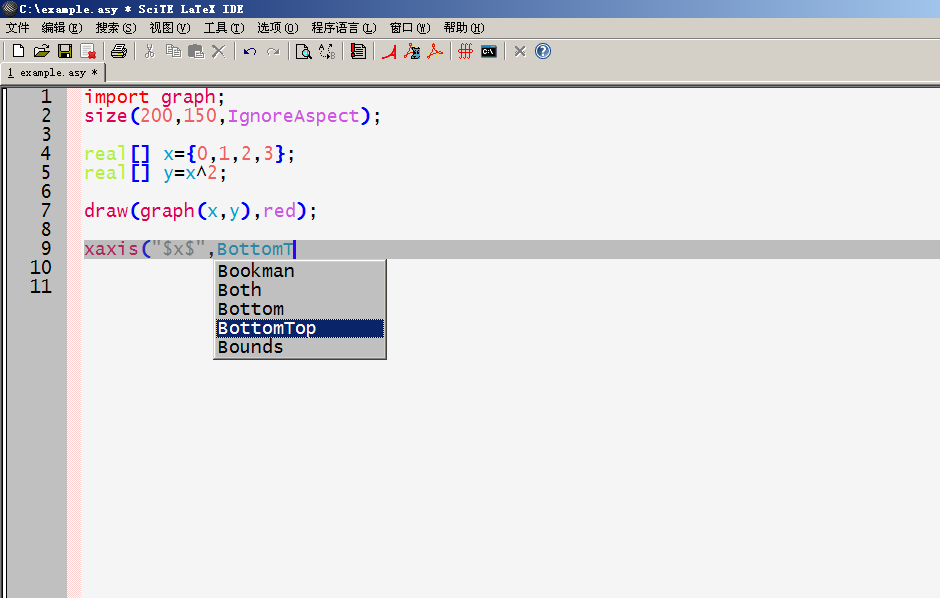
\includegraphics[width=0.6\textwidth]{SciTE.png}
\end{center}
其中那个 |asy.api| 几乎包括了 Asymptote 所有的关键词, 它可以利用
asy-keywords.el 生成的. 由于 asy-keywords.el 是随着版本更新而更新的,
因此, 如果我们希望用上最新的关键词, 可以进行如下操作来更新那个
|asy.api|.

\lstinputlisting{asyapi.asy}

把上述代码保存为 |asyapi.asy| 文件, 让它与 |C:\Program Files\Asymptote|
目录下的 |asy-keywords.el| 放在一起, 然后执行(或双击执行)
\begin{verbatim}
asy asyapi.asy
\end{verbatim}
那么就会在当前目录生成 |asy.api| 这个文件, 把它复制到 LaTeXIDE 的
SciTE.exe 所在目录就可以了.

\subsection{用 NotePad++ 编辑器}
NotePad++ 语法高亮和自动补全关键词的效果如图所示.
\begin{center}
  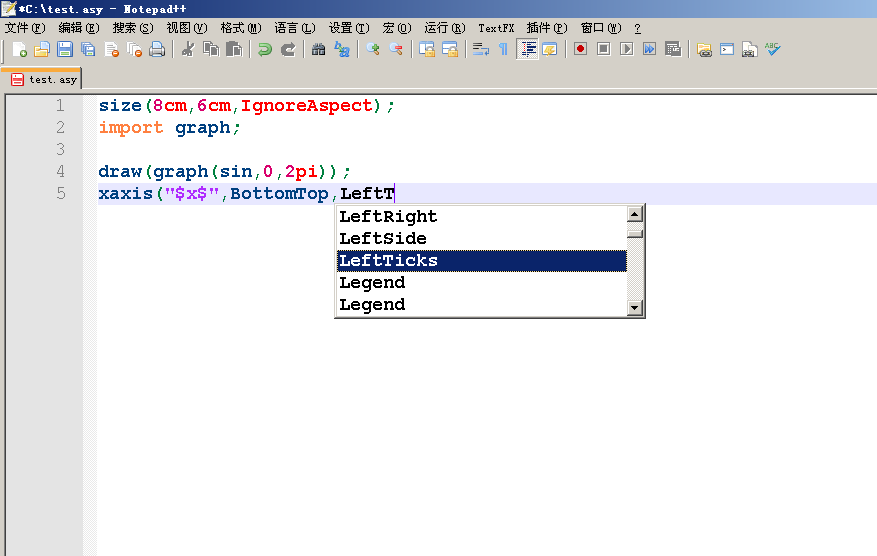
\includegraphics[width=0.6\textwidth]{NotePad++0.png}
\end{center}
ollydbg 做了一个关于本配置非常漂亮的视频, 已经打包在
\url{http://code.google.com/p/asy4cn/downloads/list} 的
ollydbg.tar.gz 中.

\subsubsection{配置 NotePad++ 的 asy 语法高亮和自动补全}
我们可以用 asy 自身来生成那个 |userDefineLang.xml| 文件, 方法如下.
在 \url{http://code.google.com/p/asy4cn/downloads/list} 的
|NotesOnAsy-*.tar.gz| 里面找到 |userDefineLangxml.asy| 这个
文件, 让它与 |C:\Program Files\Asymptote| 目录中的 |asy-keywords.el|
放在同一目录下, 接着在命令行下执行(或双击执行)
\begin{verbatim}
asy userDefineLangxml.asy
\end{verbatim}
那么就会在当前目录生成 |userDefineLang.xml| 文件, 把它复制到
|C:\Documents and Settings\ 您的用户名 \Application Data\Notepad++|
目录下. 如果一切正常, 那么重新打开 NotePad++, 这时应该在 \emph{语
  言}(Language)的最下方出现 asy, 我们把它选上. 现在我们可以用
NotePad++ 打开一个以 |asy| 为扩展名的文件, 那么就会有语法高亮显示.(注
意, 如果是采用绿色版本的 NotePad++, 那么直接把 |userDefineLang.xml| 放在
解压后 |notepad++.exe| 所在目录就可以了)

类似的, 在 \url{http://code.google.com/p/asy4cn/downloads/list}
的 |NotesOnAsy-*.tar.gz| 里面找到 |asyxml.asy| 这个文件, 把上述代码
复制进去, 让它与 |C:\Program Files\Asymptote| 中的 |asy-keywords.el|
放在同一目录下, 再执行(或双击执行)
\begin{verbatim}
asy  asyxml.asy
\end{verbatim}
同样, 会在当前目录生成 |asy.xml| 文件, 把它复制到
|C:\Program Files\Notepad++\plugins\APIs| 目录下(或 NotePad++ 那个绿色
版本的相应的目录)

接下去我们还要选择启用自动补全这个功能. 这时依次选择  \emph{设
  置}(Settings), \emph{首选项}(Preferences), \emph{备份与自动完
  成}(Backup /Auto-completion), \emph{所有输入均启用自动完成}(Enable
Auto-completion on each input) 中, 把 \emph{函数自动完成}(Function
completion) 项选上. 重新打开 NotaPad++, 我们可以试试输入一些代码, 这
时将会有代码提示, 可以用 |Enter| 和 |Tab| 选择和补全.

\subsubsection{配置 NotePad++ 编译当前 asy 文件}
\begin{center}
  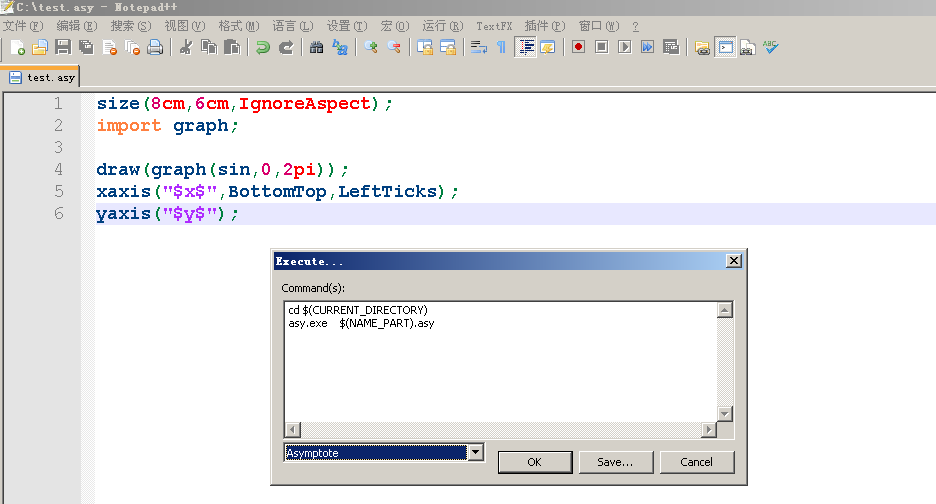
\includegraphics[width=0.6\textwidth]{NotePad++x.png}
\end{center}
编辑完 |asy| 后, 如何希望编译当前的 |asy| 文件, 那么可以选择
\emph{插件 }(Plugins), \emph{NppExec}, \emph{Execute F6} 或直接用 F6,
然后在弹出窗口填上
\begin{verbatim}
cd $(CURRENT_DIRECTORY)
asy.exe    $(NAME_PART).asy
\end{verbatim}
\begin{center}
  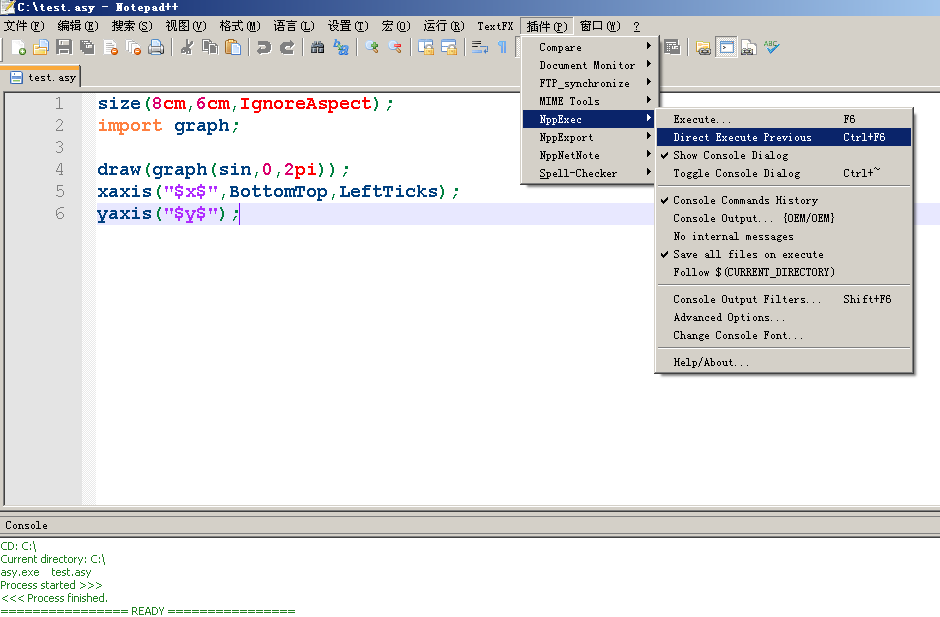
\includegraphics[width=0.6\linewidth]{NotePad++y.png}
\end{center}
然后我们把 \emph{Save all files on execute} 等勾上, 那么在编译之前就会
自动保存当前文档. 注意, 我们还可以用 |Ctrl+F6| 重复执行上一次的编译命
令. 不妨给刚才的编译命令起一个名字, 比如 |Asymptote|, 保存好下次还可以
再调用. 另外, 那个 F6 和 Ctrl+F6的这种快捷键的绑定是可以在 \emph{设
  置}(Settings), \emph{管理快捷键}(Short Mapper), \emph{Plugin
  commands}(Plugin commands) 里面更改的.

\subsubsection{配置 NotePad++ 定位语法出错行}
\begin{center}
  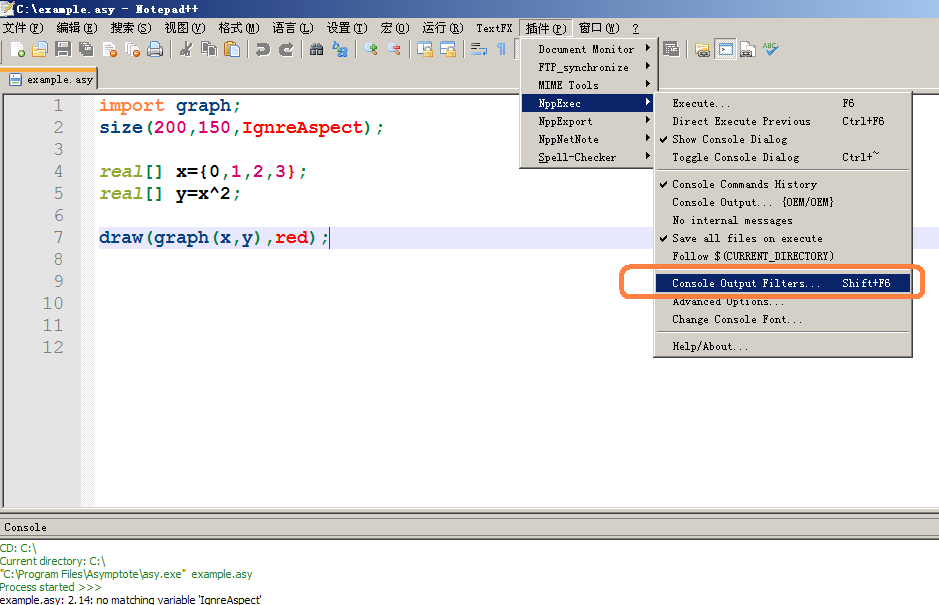
\includegraphics[width=0.6\textwidth]{NotePad++a.png}
\end{center}
我们依次点 \emph{插件}, \emph{NppExec}, \emph{Console Output Filter},
进入设置栏.
\begin{center}
  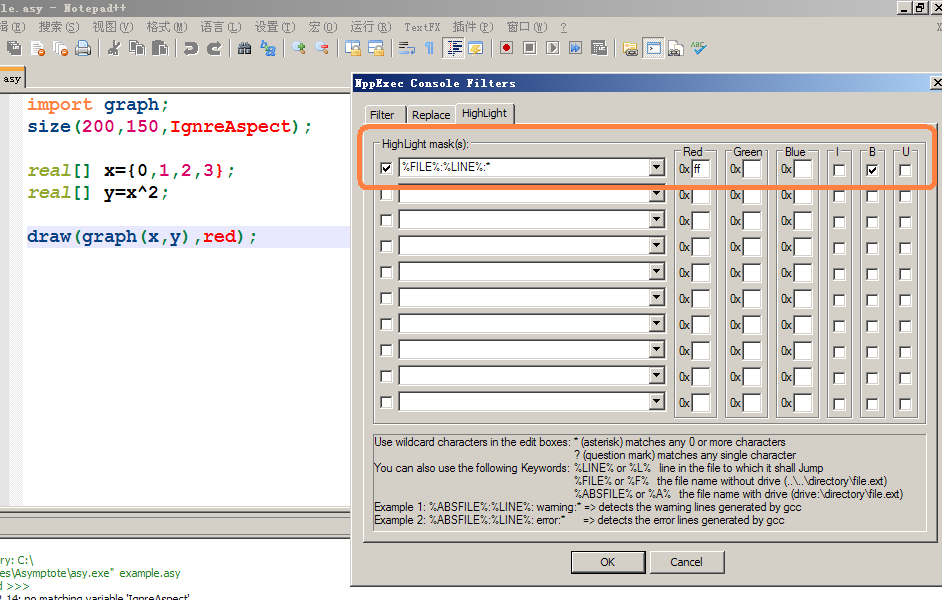
\includegraphics[width=0.6\textwidth]{NotePad++b.png}
\end{center}
因为我们观察到 asy 的出错信息的格式是
\begin{verbatim}
文件名.asy : 行数.列数 : 警告信息
\end{verbatim}
因此, 我们在第一行填上
\begin{verbatim}
%FILE%.asy:%LINE%:*
\end{verbatim}
依次代表带扩展名的文件名, 出错的行数, 警告信息. 然后选上颜色. ( 我们这
里选了红色 FF 00 00  和粗体 B)
\begin{center}
  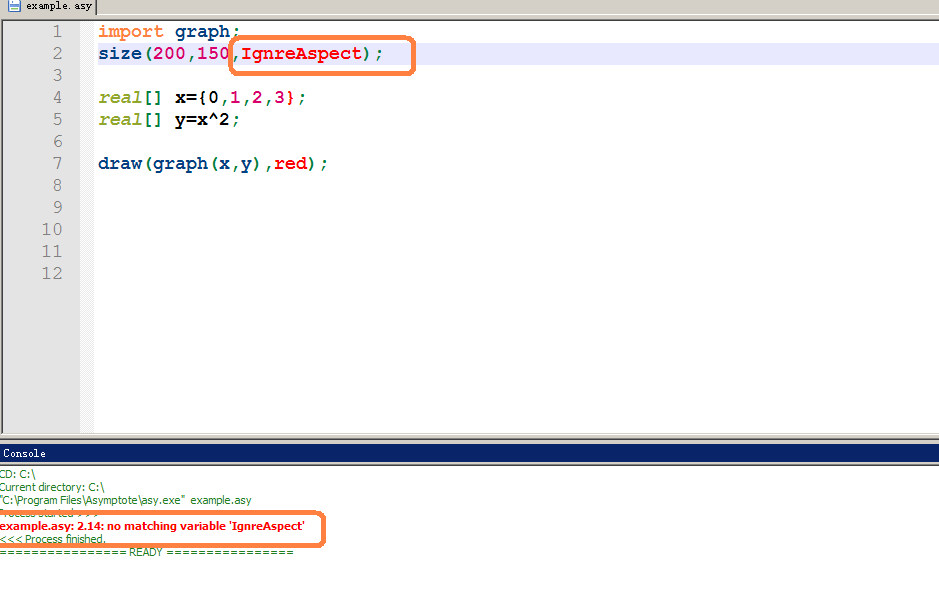
\includegraphics[width=0.6\textwidth]{NotePad++c.png}
\end{center}
\emph{双击}出错信息就会跳的源文件相应的那一行. 显然, 这个功能非常方便于我们查错!

\subsubsection{配置 NotePad++ 编译嵌入 asy 代码的 tex 文件}
类似地, 我们可以编译一个嵌入了 |asy| 代码的 |tex| 文件, 这时 F6 后填
上 (我们这里以 xelatex 为例)
\begin{verbatim}
cd $(CURRENT_DIRECTORY)
xelatex.exe  $(NAME_PART).tex
asy.exe  $(NAME_PART).asy
xelatex.exe  $(NAME_PART).tex
"C:\Program Files\Adobe\Reader 9.0\Reader\AcroRd32.exe" $(NAME_PART).pdf
\end{verbatim}
并且把它起一个名字, 确定以后就会依次用 |pdflatex|, |asy|, |pdflatex| 编
译相应的文档, 最后用 Adobe Reader 打开生成的 pdf.

如果是希望用 gsview32.exe 预览 pdf, 那么把上面做法中的最后一行如下改
动, 因为 gsview32.exe 似乎比较特殊.
\begin{verbatim}
cmd /k "C:\Program Files\Ghostgum\gsview\gsview32.exe" $(NAME_PART).pdf &EXIT
\end{verbatim}

\section{卸载}
对 Linux i386 可执行发行版本, 可以执行
\begin{verbatim}
tar -zxvf asymptote-x.xx.i386.tgz  |  xargs  --replace=%  rm /%
texhash
\end{verbatim}
其中 |x.xx| 是版本号.

如果是从源代码编译的, 请进入该目录, 然后执行
\begin{verbatim}
sudo make uninstall
\end{verbatim}


\chapter{2D 绘图}

\section{基本的绘图命令}
Asymptote 的绘图基于 |draw|, |fill|, |clip| 以
及 |label| 四个原始的命令. 前三个根源于 PostScript 的绘图命令, 最后一
个用于在图形上添加字母和图形, 此处即调用了 \LaTeX 的功能.

举一个综合的例子.
\begin{center}\includegraphics[height=4cm]{Example.pdf}\end{center}%
\lstinputlisting{Example.asy}
\begin{itemize}
\item 每一个完整的命令语句以 |;| 结尾.
\item 其中 |size(200,200);| 可以理解为我们输出图形大小是 $200\times 200$
  的图形. 可以省略为 |size(200);|.
\item {unitcircle} 是 Asymptote 预定义的路径, 表示半径为 $1$ 的
  圆. 现在调用 |draw| 命令画出.
\item 同理, 其后的一句是在封闭的路径中填上黄色.
\item 最后一句是在坐标为 $(0,0)$ 处标上字母 $O$, 其中引号内的 |$O$|
  被会输送到一个 \TeX 文件中生成相应的字母, 然后再标在 $(0,0)$ 位置.
\end{itemize}

我们先试试一些简单的绘图例子, 等对 asy 语言有一定了解以后才开始学习它的
语法.

\section{画线段和点}
\begin{center}\includegraphics[scale=0.5]{Segment-Points.pdf}\end{center}%
\lstinputlisting{Segment-Points.asy}
\begin{itemize}
\item |pair| 用来声明一种称为二元组的数据类型, 表示平面坐标. 现在对 $A$,
  $B$, $C$ 同时声明, 用了逗号连接(称为逗号运算符).
\item |--| 表示用直线连接两点.
\item |dot| 用于画出一个实心点, 其后加上 |UnFill| 就得到
  空心的点. 这个 |UnFill| 真正的把点挖空, 而不是用白色填充, 这是
  Asymptote 提供的重要功能之一.
\end{itemize}

\section{画虚线}
\begin{center}\includegraphics[scale=0.5]{Dashed-Line.pdf}\end{center}%
\lstinputlisting{Dashed-Line.asy}
\begin{itemize}
\item  其中 |solid| 可以省略, 表示画实线;
\item |dashed| 画虚线.
\item |dashdotted| 画点划线.
\item |dotted| 画实心点线.
\end{itemize}
更多线的类型将在后面阐述.

\section{画箭头}
\begin{center}\includegraphics[height=6cm]{Arrows.pdf}\end{center}%
\lstinputlisting{Arrows.asy}

\begin{itemize}
\item |Arrow| 与 |EndArrow| 效果一样, 都是在路径的末端添
  加箭头.
\item |BeginArrow| 在路径的开头加箭头.
\item |Arrows| 在路径的头尾都加上箭头.
\item |MidArrow| 则是在路径的中间添加箭头.
\end{itemize}
|Arrow| 其实是一个函数, 我们可以带上一些参数控制它的大小, 形状以及安放
的位置, 这些在后面再详细论述.

Asymptote 预先定义了一些表示方向的二元组,比如  |E=(1,0)|,
|S=(0,-1)|, |W=(-1,0)|, |N=(0,1)| 以及它们的复合
|NE| 等等. 因为二元组同时也表示平面坐标系中的点, 因此, 这些方向
同时也表示点. 举一个综合一点的例子,

\begin{center}\includegraphics[scale=0.8]{Compass-1.pdf}\end{center}%
\lstinputlisting{Compass-1.asy}

其中 |label| 是 Asymptote 里面的一个函数, 用于标字母或图形, 可
以事先指定标的位置(|position|) 以及相对与那个位置的放法(|align|), 因此, 该函
数的调用格式之一是:
\begin{verbatim}
label(Label,position,align);
\end{verbatim}
如最后一行我们把 $NE$ 这个 |Label| 标在 |position=NE| 这个点的东北
(|align=NE|).

从刚才那个例子, 我们可以初步了解到 Asymptote 中的函数都可以加上一些数
据, 我们把这些数据称为该函数的\emph{参数}. 另外, 函数也可以复合. 比如
我们可以让 |draw| 和 |Label| 函数复合, 以便同时画方向以及在其实标字母.
\begin{center}\includegraphics[scale=0.8]{Compass-2.pdf}\end{center}%
\lstinputlisting{Compass-2.asy}
当然, 更为重要的时, 我们可以同时控制 |Label| 与 |draw| 的关系, 从而达
到把 |Label| 标在我们希望的位置. 特别的, 看最后一行, |position=EndPoint| 表明
我们把 |Label| 标在路径 |O--WNW| 的末端.

\section{画线段按比例的分点}
对两个点 $A$ 和 $B$ 构成的线段(我们后面称为 {path} 的数据类型),
我们可以用 |midpoint| 函数来求它们的中点.
调用格式是:|midpoint(path)|

\begin{center}\includegraphics[scale=0.6]{Midpoint.pdf}\end{center}%
\lstinputlisting{Midpoint.asy}

其中 |--cycle| 表示我们用 |--| 这种连接方式使得所画的路
径是封闭而且是周期循环的.特别要注意的是: |A--B--C--cycle| 与
|A--B--C--A| 是不一样的. 后者并不形成一个封闭路径, 它只是一条首尾
巧好是同一个点的路径.因此, 也只有前者才可以在有它围成的封闭区域填上
颜色.那个 |filldraw| 就是把路径填上颜色的同时把该路径围成的封闭
区域也填上颜色.这两个颜色可以不一样.
\begin{center}\includegraphics[scale=0.5]{FillDraw.pdf}\end{center}%
\lstinputlisting{FillDraw.asy}

一般的, 我们用 |T interp(T a, T b, real t)| 表示
|a+t*(b-a)|, 即从 |a| 往 |b| 方向走到占整段比
例为 |t| 的地方, 于是当比例 |t=1/2| 是就是中点. 另外,
|T| 可以代任意有加减乘运算的一些诸如 |real|,
|pair| 等的数据类型.
\begin{center}\includegraphics[scale=0.6]{Interp.pdf}\end{center}%
\lstinputlisting{Interp.asy}

\section{画过若干个点的曲线}
用 |..| 表示这种
与直线不一样的连接两个点方式. 这种画曲线原理将在后面讲到.

现在我们可以利用四个点 $E$, $N$, $W$, $S$ 来画出一个与圆非常接近的图形.
\begin{center}\includegraphics[scale=0.5]{Circle.pdf}\end{center}%
\lstinputlisting{Circle.asy}

下面我们利用曲线功能画一些有趣一点的图形.
\begin{center}\includegraphics[scale=0.5]{Heart.pdf}\end{center}%
\lstinputlisting{Heart.asy}

\section{变量与函数}
我们在前面其实已经接触到\emph{变量}和\emph{函数}这两个概念, 在这里阐述
一下. Asymptote 中的\emph{变量}就是在使用之前要预先定义好的数据类型. 比如前
面的表示方向的 |E|, |N|, |W|, |S| 以及各种
颜色 |red|, |green| 等等. 用户也可以自定义一些变量,但一
定要事先声明它的数据类型. 这种语法与 C++/Java 是类似的(但本书不假定读者
学过任何语言).至于 \emph{函数}, 在 Asymptote 中也把它看成变量, 我们说它是一种一阶变
量, 于是普通的 \emph{变量} 就可以看成零阶变量, 两个函数复合就是更高阶的
变量. 这是 Asymptote 语言最为独特的一点, 也使得我们在函数中调用或定义函
数非常方便. Asymptote 预先定义了很多画基本图形的函数, 可以直接调用, 不过我们心里面
要清楚函数需要的参数是什么.这些常用的函数包括(后面会看到, 如果调用
\begin{itemize}
\item {box(矩形的左下角, 矩形的右上角);}
\item {ellipse(椭圆的中心,水平方向的轴长,竖直方向的轴长);}
\item {drawline(直线的第一个点, 直线上的第二个点);}
\end{itemize}

\begin{center}\includegraphics[scale=0.5]{Box-Circle-Ellipse.pdf}\end{center}%
\lstinputlisting{Box-Circle-Ellipse.asy}

\section{画正多边形}
\begin{center}\includegraphics[scale=0.5]{Polygon.pdf}\end{center}%
\lstinputlisting{Polygon.asy}

\section{画圆弧}
圆弧是圆的一部分, 用 |arc| 函数.
\begin{lstlisting}
  path arc(pair c, real r, real angle1, real angle2);
\end{lstlisting}

\begin{center}\includegraphics[scale=0.5]{Arc.pdf}\end{center}%
\lstinputlisting{Arc.asy}

其中 |defaultpen(linewidth(4));| 把默认的画笔的设为 |4bp| 粗细.

有时候我们希望画一个角之间的圆弧, 比如通常的平面几何的图形中给角做一个
标记, 默认的作图没有这个功能, 这时就要调用 Asymptote 里面的 geometry 宏包.
\begin{center}\includegraphics[scale=0.5]{Angle-Mark.pdf}\end{center}%
\lstinputlisting{Angle-Mark.asy}

\section{画直角记号}
直角符号用 |perpendicular| 函数,同样要调用 |geometry| 宏
包. 基本的用法是
\begin{verbatim}
perpendicular(pair z,pair align,pair dir);
perpendicular(pair z,pair align,path g);
\end{verbatim}
该直角是相对 |z--z+dir| 的, |align| 表明它的安置的方位,
给出路径 |g| 的话, Asymptote 会把它转成该路径 |g| 的切线
方向(关于路径的切线方向我们以后阐述).
\begin{center}\includegraphics[scale=0.5]{Perpendicular.pdf}\end{center}%
\lstinputlisting{Perpendicular.asy}

\section{自定义函数}
我们也可以自己定义新函数. 假定我们要画一条抛物线 $y=x^{2}$, 我们要预先定义一个函数. 格式如下
\begin{lstlisting}
  real f(real x){return y=x^2;};
\end{lstlisting}
其中 |real x| 声明函数自变量 |x| 是实数型, |f| 前面的
|real| 声明函数 |f| 也是一个实数型.

\section{画参数曲线}
利用若干个点画曲线能力有限, 我们可以利用数学中的参数曲线来生成更丰富多
彩而且有意义的曲线.
\begin{center}\includegraphics[scale=0.5]{Parameter-Curve-1.pdf}\end{center}%
\lstinputlisting{Parameter-Curve-1.asy}

函数 |graph| 是一个返回数据类型为路径 |path| (其实是称为 |guide| 的
数据类型, 与 |path| 稍微有些区别)的函数.它需要知道要画的函数
|real f(real x)|,  所画函数自变量的变换范围, 还有就是用折线画
还是用光滑曲线画.因此, 前面代码调用它的格式如下:
\begin{lstlisting}
  guide graph(real f(real), real a, real b,interpolate join=operator --);
\end{lstlisting}
\begin{center}\includegraphics[scale=0.8]{Parameter-Curve-2.pdf}\end{center}%
\lstinputlisting{Parameter-Curve-2.asy}

\begin{itemize}
\item 在 |Label()| 函数中加 |position=EndPoint|,那么就
  会标在所画曲线的末端, 也可以用完全等价的 |position=Relateve(1)|.
\item  类似地,标 $y$ 轴时用 |align=N| 把 $y$ 安置(|align|)在 $y$ 轴默认的
  |position=EndPoint| 的北边.
\end{itemize}

\section{画阴影}
传统的图形, 特别是印成黑白颜色的图形, 通常是希望在封闭曲线里面填上阴影
而不是颜色. Asymptote 的宏包 {patterns} 提供了一些模式, 我们先
讲最常见的一种 hatch 画阴影.
\begin{center}\includegraphics[scale=0.5]{Hatch.pdf}\end{center}%
\lstinputlisting{Hatch.asy}
\begin{itemize}
\item {hatch(NW)} 是一种西北走向的阴影斜线的图形. 用
  |add("name",hatch(NW));| 命名为 "name".
\item 接下去用 |pattern("name")| 的方式把它做成一个类似与颜色的
  画笔.
\item |hatch()| 函数还有其他参数, 比如线的粗细, 线的间隔等.
\end{itemize}

\section{子图}
在 Asymptote 中我们可以独立的画一些图, 然后再分别添加到图上.这时,我们
可以定义一些称为 {picture} 的数据类型.
\begin{center}\includegraphics[scale=0.5]{Sub-Picture-1.pdf}\end{center}%
\lstinputlisting{Sub-Picture-1.asy}

这与直接画的效果似乎是一样的, 不过用这种独立画的方式的其中一个便利的地
方是可以随意控制图片的画出顺序.这时候用 {above=true} 和 {above=false}
控制的.
\begin{center}\includegraphics[scale=0.5]{Sub-Picture-2.pdf}\end{center}%
\lstinputlisting{Sub-Picture-2.asy}

我们看到, 现在最后加上的图反而给前面画的图盖住了. 这种灵活的独立图形的
输出的是独立画图的好处之一.这个也用在下面的 |clip| 命令用法当中
以及以后的动画制作.

\section{裁剪命令 clip}
除了前面已经阐述的 |draw|,|fill|,|label| 三个基本命令以外, 还有一个
|clip| 命令, 可以借助于封闭曲线裁剪出该曲线围成的区域里面的部分.
\begin{lstlisting}
  clip(picture pic=currentpicture, path g, stroke=false, pen fillrule=currentpen);
\end{lstlisting}

\begin{center}\includegraphics[scale=0.5]{Clip-1.pdf}\end{center}%
\lstinputlisting{Clip-1.asy}

利用 |clip| 这个函数, 我们可以任意地裁剪出我们所想要的东西, 然后再用
|add| 函数添加.
\begin{center}\includegraphics[scale=0.5]{Clip-2.pdf}\end{center}%
\lstinputlisting{Clip-2.asy}

我们定义了一个子图 |pic| 用来独立画一个虚线单位圆, 然后用路径
|p| 把它剪下来. 最后再用 |add| 添加到图上.

下面的 Venn 图的例子运用上面技巧画出了两个集合交集部分的.
\begin{center}\includegraphics{Clip-3.pdf}\end{center}%
\lstinputlisting{Clip-3.asy}

\section{unfill 命令}
Asymptote 利用 |clip| 这个功能定义了一个非常好用的 |unfill| 命令, 可以
利用封闭曲线来挖洞. 前面我们已经见过 |UnFill|, 再举一个例子.

\section{奇偶法则填颜色}

我们前面已经看到 {fill} 命令可以在封闭循环的路径内填上各种颜色.
\begin{center}\includegraphics[scale=0.6]{EvenOdd.pdf}\end{center}%
\lstinputlisting{EvenOdd.asy}
\section{变换}
变换可以使得我们可以利用原来的图形来生成新的图形. Asymptote 可以进行一
般的仿射变换, 即可以进行旋转, 伸缩, 旋转, 反射等变换以及它们的复合.

平移变换是
\begin{lstlisting}
  transform shift(real x,real y);
  transform shift(pair z);
\end{lstlisting}
分别为依照向量 |(x,y)| 和 |z| 平移.

\begin{center}\includegraphics[scale=0.6]{Shift.pdf}\end{center}%
\lstinputlisting{Shift.asy}

伸缩变换包括
\begin{lstlisting}
  transform xscale(real x);
  transform yscale(real y);
  transform scale(real s);
  transform scale(real x, real y);
\end{lstlisting}

\begin{lstlisting}
  transform slant(real s);
\end{lstlisting}

错切变换 |slant| 变换把点 |(x,y)| 变换为 |(x+s*y,y)|.
\begin{center}\includegraphics[scale=0.8]{Slant.pdf}\end{center}%
\lstinputlisting{Slant.asy}
从图中可以看到, 点 |(0.5,0.5)| 经过错切 |slant(2)| 变换后变成点
|(1.5,0.5)|. 经过简单的运算, 我们可以知道 $s=\tan\alpha$, 其中
$\alpha$ 是错切变换 |slant| 的倾斜角.

\begin{lstlisting}
  transform rotate(real angle, pair z=(0,0));
\end{lstlisting}
旋转变换 |rotate| 是绕着点 |z| 旋转 |angle| 度数. 默认是绕着坐标原点旋
转.
\begin{center}\includegraphics[scale=0.8]{Rotation.pdf}\end{center}%
\lstinputlisting{Rotation.asy}

\begin{lstlisting}
  transform reflect(pair a, pair b);
\end{lstlisting}
反射变换是以 |a--b| 这条直线为对称轴反射.


\section{简单的编程}
Asymptote 的语法类似于 C, C++, 以及 Java. 不过本书不假定读者有任何的编
程语言背景, 反而是希望直接学习 asy 这种有趣的绘图语言.

我们在前面已经接触了它的一些语法, 这里归纳一下.首先, 每一个\emph{变量}都要声
明它的数据类型.比如

\begin{lstlisting}
  real x;
  pair z;
\end{lstlisting}
然后对应地赋予相应的值.
\begin{lstlisting}
  x=1.0;
  z=(3.0,4.0);
\end{lstlisting}

最后,就是一些程序设计语言都有的判断语句和循环语句.我们在这里说一下用
的最多的 |for| \emph{循环语句}.

假定我们要画半径分别为 $1$, $2$, $3$,...
的几个同心圆, 我们当然可以如下画出:
\begin{center}\includegraphics[scale=0.6]{Circle-3.pdf}\end{center}%
\lstinputlisting{Circle-3.asy}

这也未尝不可, 可是再要求多画几个,大家也就会觉得烦了. 编程语言都提供一种
叫 |for| 循环的语句去干这个事情.

\begin{center}\includegraphics[scale=0.6]{For-Circle.pdf}\end{center}%
\lstinputlisting{For-Circle.asy}

我们解释一下 |for| 括号里面三个语句的意思.
\begin{itemize}
\item 第一个语句 |int i=1;| 是对变量 |i| 赋予初始值
  |1|;
\item 第二个语句 |i<4;| 是判断 |i| 是否小于 |4|,
  如果是, 就执行 |draw(circle(O,i));|
\item 第三个语句  |++i| 把 |i| 增加 |1|.
\end{itemize}

按照这个规律,  与 |i=1| 对应的 |draw(circle(O,1))| 是最先执行的. 然后
|i++| 使得 |i| 从 |1| 增加到 |2|, 仍然满足 |i<4| 这个的条件, 因此, 接
下去可以执行 |i=2| 对应的 |draw(circle(O,2))|. 做完以后把 |i++| 又使得
|i| 从 |2| 增加到 |3|, |i=3| 对应的 |draw(circle(O,3))| 被执行. 最后,
变量 |i| 增加到 |4|. 由于此时 |i| 已经增加到了 |4|, 不再满足 |i<4|
的条件, 因此|for| 就此停止工作.

我们看到, 现在也是恰好画了半径分别为 |i=1|, |i=2|,|i=3| 的三个同心圆,
是不是很神奇!

下面再列举一些简单的例子.
\begin{center}\includegraphics[scale=0.6]{For-Dots.pdf}\end{center}%
\lstinputlisting{For-Dots.asy}

\begin{center}\includegraphics[scale=0.6]{For-Ellipses.pdf}\end{center}%
\lstinputlisting{For-Ellipses.asy}

\begin{center}\includegraphics[scale=0.6]{For-Grid.pdf}\end{center}%
\lstinputlisting{For-Grid.asy}

下面的例子稍微复杂一些, 即先在一个 |picture pic;| 里面画好一个基本的图
形, 然后通过平移达到铺砌平面.
\begin{center}\includegraphics[scale=0.8]{For-Square.pdf}\end{center}%
\lstinputlisting{For-Square.asy}

由于循环的应用大部分是与数组结合起来的, 因此我们后面还有讨论一下数组以
及它的应用, 到时候我们有更为精彩的例子可以介绍.

\section{与向量 pair  有关的一些函数}
我们先归纳一下与向量 pair 这种数据类型有关的一些知识.

\begin{typelist}
\item[int] 整数类型; 如果没有给定初始式, 默认值为 |0|. 整数允许的最小值
  为 |intMin|, 最大值为 |intMax|. 我们可以用
  \begin{lstlisting}
    write(intMin);
    write(intMax);
  \end{lstlisting}
  看看这两个数.

\item[real] 实数; 它将设为计算机结构的本地浮点类型的最大精度. 实数的隐式
  初始式为 |0.0|. 实数具有精度 |realEpsilon|, 有效数字为 |realDigits|. 最小的
  正实数为 |realMin|, 而最大的正实数为 |realMax|.

\item[pair] 向量, 也看成是复数, 实数构成的有序对 |(x, y)|. 复数 |z| 的实部和虚部可读为
  |z.x| 和 |z.y|. 我们称 |x| 和 |y| 为复数数据元素的虚拟成员; 然而, 它们不能
  直接修改. 复数的隐式初始式为 |(0.0,0.0)|.

  \begin{funclist}
  \item |pair conj(pair z)| \go
    返回 |z| 的复共轭.

  \item |real length(pair z)| \go
    返回向量 |z| 的长度, 即复数的模.
  \item |real abs(pair z)|\go
    与 |length(pair)| 功能一样.

  \item |real angle(pair z)| \go
    返回 |z| 的幅角, 单位为弧度, 在区间 $[-\uppi, \uppi]$ 内取值.

  \item |real degrees(pair z, bool warn=true)| \go
    返回 |z| 的幅角, 单位为度, 在区间 $[0,360)$ 内, 当 |warn| 为 |false| 且
    |z.x=z.y=0| 时返回 |0|(而不是产生错误). 这个 |warn=flase| 可以在与
    极坐标互相转换时避开 |(0,0)| 这个奇点.

  \item |pair unit(pair z)| \go
    返回与复数 |z| 同方向的单位向量.

  \item |pair expi(real angle)| \go
    返回以弧度角 |angle| 为方向的单位向量, 这里用 |expi| 这个符号是源于
    $e^{i\theta}$.

  \item |pair dir(real degrees)| \go
    返回以角度 |degrees| 为方向的单位向量,

  \item |real xpart(pair z)| \go
    返回 |z.x|.

  \item |real ypart(pair z)| \go
    返回 |z.y|.

  \item |real dot(pair z, pair w)| \go
    返回点积 (内积) |z.x*w.x+z.y*w.y|

  \item |pair minbound(pair z, pair w)| \go
    返回 |(min(z.x,w.x),min(z.y,w.y))|.

  \item |pair maxbound(pair z, pair w)| \go
    返回 |(max(z.x,w.x),max(z.y,w.y))|.
  \end{funclist}

\end{typelist}

\section{Bezier 曲线的原理及与 path 有关函数}
Asymptote 画曲线与通常的其他软件不一样, 并非采用折线逼近来生成曲线的
办法, 而是采用一种称为 Bezier 曲线办法. 我们在此花一些篇幅来介绍这个概
念. 因为一旦我们理解 Asymptote 这种生成曲线或曲面的方法, 将会有助于我
们理解 Asymptote 的与路径 |path| 相关的一些命令, 做到心中有数, 也有助
于灵活地解决问题.

我们前面已经懂得如何画直线段, 如何生成曲线呢? 1959 年, 法国人 Paul de
Casteljau(与此独立地, 1962 年的 Bezier) 发现了现在称为 Bezier 曲线的生
成光滑曲线的办法. 我们在此阐述一下其中巧妙的想法.

\begin{center}\includegraphics{Bezier-Principle-1.pdf}\end{center}%
\lstinputlisting{Bezier-Principle-1.asy}

给出 $Z_{0}$ 和 $Z_{1}$ 两个点, 我们只能得到连接它们的直线段, 此时如果
给出一个时刻 |t|, 那么我们可以通过这个时刻访问到这条线段上以 $t$
为比例的点, 即 $(1-t)Z_{0}+t Z_{1}$. de Casteljau 天才的想法是添加一个额
外的点 $C$, 并且把它称为控制点. 然后我们顺次连接 $Z_{0}$, $C$, $Z_{1}$, 只
能得到一段折线, 下面我们按照一个比例 $t$ (我们也称为时刻 $t$), 比如
$t=\frac{1}{3}$, 然后在 $Z_{0}$ 到 $C$ 的 $\frac{1}{3}$ 处取一个点
$A$, 同样, 在 $C$ 到 $Z_{1}$ 的 $\frac{1}{3}$ 处取另外一个点 $B$, 连接 $A$
与 $B$, 然后在 $A$ 到 $B$ 的 $\frac{1}{3}$ 处再取点 $Z$, 那么就称 $Z$
为对应于这个时刻 $\frac{1}{3}$ 一个点. 我们可以想象, 当那些时刻遍历
$0$ 到 $1$ 的所有的时刻, 就得到一条轨迹, 通过简单的代数运算, 我们可以
依次得到
\begin{gather}
  A=(1-t)Z_{0}+tC \label{one}\\
  B=(1-t)C+tZ_{1}\label{two}\\
  Z=(1-t)A+tB\label{three}
\end{gather}
把 \eqref{one} 和 \eqref{two} 代入 \eqref{three}, 我们可以得到 $Z$ 与
$t$ 的关系.
\begin{displaymath}
  Z(t)=(1-t)^{2}Z_{0}+2t(1-t)C+t^{2}Z_{1}
\end{displaymath}
这是一条过 $Z_{0}$ 和 $Z_{1}$ 的二次参数曲线.
% 这种 BeZier 曲线有许多良好的性质, 比如我们可以不用真正的遍历 $0$ 到
% $1$ 之间的所有时刻, 只需按照计算机通常的迭代办法, 分别就刚才的
% $Z_{0}$, $A$, $Z$ 与 $Z$, $B$, $Z_{1}$ 重复刚才的做法(那个比例 $\frac{1}{3}$
% 固定), 又可以得到其他两个该曲线上的点, 这样做足够多却是有限多次, 就能
% 生成一条肉眼看起来是连续的曲线.

我们上面得到的是 $2$ 次的参数曲线, 如果采用两个控制点, 那么我们就能得
到 $3$ 次的 Bezier 曲线, 其中的原理是类似的,  请观察图.
\begin{displaymath}
  (1-t)^{3}z_{0}+3t(1-t)^{2}c_{0}+3t^{2}(1-t)c_{1}+t^{3}z_{1}
\end{displaymath}
Asymptote 里面就是采用这种 $3$ 次曲线. 我们可以把这种生成曲线的方式推
广到曲面.
% 而且这种\emph{逐点}的方式非常有利用我们以后产生光滑渐
% 变的染色效果(请参见后面 3D 曲面的颜色渐变效果部分)

\begin{center}\includegraphics[scale=1.2]{Bezier-Principle-2.pdf}\end{center}%
\lstinputlisting{Bezier-Principle-2.asy}

下面我们介绍一下与路径 |path| 有关的一些函数.

\begin{funclist}
  |pair precontrol(path p, int t)| \go

\end{funclist}

\begin{funclist}
  |pair postcontrol(path p, int t)| \go

\end{funclist}


\begin{funclist}
  |int length(path p)| \go
  一般的曲线是由若干条 Bezier 曲线连接起来的, 这里返回的是路径 p 的总
  的分段数目. 比如我们可以用
  |write(unitcircle);   write(length(unitcircle));|
  看看 |unitcircle| 的构造以及它的 |length|.

\end{funclist}

\begin{funclist}
  |pair point(path p,real t)| \go
  我们在前面已经介绍了 Bezier 曲线的生成原理, 从中我们可以知道, 对于一条
  这种两个控制点的 3 次 Bezier 曲线, 随便给出一个时刻 |t|, 我们是可以很
  简单的得出时刻 |t| 对应的点.
\end{funclist}

\begin{center}\includegraphics{Precontrol-Postcontrol.pdf}\end{center}%
\lstinputlisting{Precontrol-Postcontrol.asy}

\section{数组}
我们经常要表示一列对象 $A_{0}$, $A_{1}$, $A_{2}$, $\cdots$, 它们具有相同
的类型.

\section{subfigure}
\begin{center}\includegraphics[scale=0.8]{Subfigure.pdf}\end{center}%
\lstinputlisting{Subfigure.asy}

\section{graph 宏包}
\begin{center}\includegraphics[scale=0.8]{Graph-Test-3.pdf}\end{center}%
\lstinputlisting{Graph-Test-3.asy}
\begin{center}\includegraphics[scale=0.8]{Graph-Test-2.pdf}\end{center}%
\lstinputlisting{Graph-Test-2.asy}

\section{极坐标}
\begin{center}\includegraphics[scale=0.8]{Polar-Coordinate.pdf}\end{center}%
\lstinputlisting{Polar-Coordinate.asy}

\section{数项级数表示的函数}
\begin{center}\includegraphics[scale=0.8]{Series-1.pdf}\end{center}%
\lstinputlisting{Series-1.asy}
首先, 我们要定义一个函数族 $f_{n}(x)$, 为此我们定义与 |n| 相关的函数
|f(n)|, 由于函数是一种实型返回实型的数据类型, 这个不是已经有的类型, 因
此我们需要用 |typedef| 定义这种新的数据类型, 我们给它一个 |func| 的名
称.

接下去用匿名函数 |new| 新建一个实型返回实型的函数, 然后返回函数 |f(n)|
的表达式. 过程有些曲折, 不过这是因为 Asymptote 把函数也当成变量来处理
的缘故.
\begin{center}\includegraphics[scale=0.8]{Series-2.pdf}\end{center}%
\lstinputlisting{Series-2.asy}

\section{分段函数}
\begin{center}\includegraphics[scale=0.8]{Piecewise-Function.pdf}\end{center}%
\lstinputlisting{Piecewise-Function.asy}

\section{画线程图}
\begin{center}\includegraphics[scale=0.8]{Flows.pdf}\end{center}%
\lstinputlisting{Flows.asy}

\section{读入数据绘图}
假定我们有一些点的坐标, 我们有两种方法读入这些数据后绘图.

\begin{lstlisting}
  96.25		3.00239
  96.00		2.99448
  95.95		2.99289
  95.90		2.9913
  95.85		2.9897
  95.80		2.98809
  95.75		2.98645
  95.72		2.98545
  95.71		2.98509
  95.71		2.98493
  95.72		2.98519
  95.75		2.98601
  95.80		2.98743
  95.85		2.98885
  95.90		2.99028
  95.95		2.99169
  96.00		2.99309
  96.05		2.99446
  96.10		2.99577
  96.15		2.99696
  96.16		2.99716
  96.17		2.99734
  96.18		2.99746
  96.185	2.99746
  96.188	2.99739
  96.188	2.99706
  96.185	2.99676
  96.18		2.9964
  96.17		2.99578
  96.16		2.99521
  96.15		2.99466
  96.10		2.99205
  96.05		2.98944
  96.00		2.98671
  95.95		2.98376
  95.90		2.9804
  95.85		2.97619
  95.84		2.97513
  95.83		2.97392
  95.82		2.97248
  95.81		2.97054
  95.805	2.96901
  95.805	2.96463
  95.81		2.96307
  95.82		2.9611
  95.83		2.95962
  95.84		2.95838
  95.85		2.95729
  95.90		2.9529
  95.95		2.94939
  96.00		2.94631
  96.25		2.93356
\end{lstlisting}
\begin{center}\includegraphics[scale=0.8]{filegraph.pdf}\end{center}%
\lstinputlisting{filegraph.asy}

另外一种做法如下.
\lstinputlisting{Data.asy}

\section{各种循环语句}
\begin{center}\includegraphics[scale=0.8]{Cyclic-Star.pdf}\end{center}%
\lstinputlisting{Cyclic-Star.asy}

\section{弯曲路径上标标签}
\begin{center}\includegraphics[scale=0.8]{Label-Curve-1.pdf}\end{center}%
\lstinputlisting{Label-Curve-1.asy}
\begin{center}\includegraphics[scale=0.8]{Label-Curve-2.pdf}\end{center}%
\lstinputlisting{Label-Curve-2.asy}
\begin{center}\includegraphics[scale=0.8]{Label-Curve-3.pdf}\end{center}%
\lstinputlisting{Label-Curve-3.asy}

\section{随机}
\begin{center}\includegraphics{Random.pdf}\end{center}%
\lstinputlisting{Random.asy}

\section{模拟徒手绘图的效果}
Ivaldi 提供的 |trembling| 宏包可以模拟徒手绘图, 比较有趣.
\begin{center}\includegraphics[scale=0.8]{Tremble.pdf}\end{center}%
\lstinputlisting{Tremble.asy}
\section{分形图}
\begin{center}\includegraphics[scale=0.8]{Fractal.pdf}\end{center}%
\lstinputlisting{Fractal.asy}
下面画树的代码是从 \emph{Learning METAPOST by Doing} 的 \MP{} 代码翻译
过来的.

\begin{center}\includegraphics{Tree.pdf}\end{center}%
\lstinputlisting{Tree.asy}

我们也可以把 examples 目录下的  |PythagoreanTree.asy| 改编一下, 只画出
一层绿色的叶子.
\begin{center}\includegraphics{PythagoreanTree-new.pdf}\end{center}%
\lstinputlisting{PythagoreanTree-new.asy}

\section{动画}
Asymptote 的动画分 gif 和 mpeg 以及 pdf 三种格式, 前面两种都是调用
ImageMagick 把若干张 eps 或 pdf 图片经过转换以后叠合起来, 而 pdf 格式
的则是调用 LaTeX 的 animation 宏包去完成这个叠合与嵌入任务的.

我们先举 pdf 的例子. Asymptote 通过 |animate| 宏包调用 LaTeX 的
|animation| 宏包, 我们需要用 |import animate|, 然后定义一个数据类型为
|animation| 的 Ani.
\begin{center}
\begin{asy}
import animate;
pair[] P={(5,0),(-8,50),(55,50),(100,0)};
defaultpen(fontsize(20pt)+1.5pt);
animation Ani;
int n=30;
for(int i=0;i<n;++i){
  picture pic;
  size(pic,300);
  real t=i/n;
  pair A=interp(P[0],P[1],t);
  pair B=interp(P[1],P[2],t);
  pair C=interp(P[2],P[3],t);
  pair U=interp(A,B,t);
  pair V=interp(B,C,t);
  pair W=interp(U,V,t);
  draw(pic,P[0]--P[1]--P[2]--P[3]);
  draw(pic,A--B--C,green);
  draw(pic,U--V,blue);
  draw(pic,P[0]..controls A and U.. W,red);
  Ani.add(pic);
}
label(Ani.pdf("controls,autoplay,loop",keep=true,delay=400));
\end{asy}
\end{center}
\lstinputlisting{Bezier-Animation.asy}

\section{做动画幻灯}
\lstinputlisting{Random-Numbers.asy}

\begin{itemize}
\item |controls| 表示我们采用控制健(包括单步, 快进, 自动播放, 调整自动
  播放速度的健等等.
\item |autoplay| 表示我们让 pdf 默认自动播放.
\item |loop| 表示在自动播放时不断循环.
\end{itemize}

\section{与 xasy 结合绘图}
\begin{center}\includegraphics[scale=0.8]{Xasy.pdf}\end{center}%
\lstinputlisting{Xasy.asy}



\chapter{3D 绘图}

\section{Asymptote 三维作图概述 }

\begin{verbatim}
首先, 请注意, 本文档代码中的出现的 ^ 是 unicode 编码, 都要手工改为
ascii 编码的 ^ .另外, 对 Windows 的用户, 如果出现 outoff memory 的出
错提示, 请在命令行加上 -compact 或 -divisor=4 选项, 也可以在代码适
当位置加上 purge(divisor=4).
\end{verbatim}

与另外一种与 \TeX 结合紧密的 metapost 语言不同, Asymptote 提供了一种原
生的方式去生成三维的曲线, 主要是把 MetaPost 作者 Hobby 关于二维情形自
动选择控制点生成曲线的方法推广到三维.

Asymptote 中与 3D 有关的主要是 three, graph3, solids  三个宏包, 其他辅
助的宏包还有 tube, grid3, contour3, obj, labelpath3 等等. 在画 3D 图形
之前, 我们一般都要调用前面三个宏包之一二.

\section{预览 3D 输出}
先给出一个简单的 3D 例子.
\begin{center}\includegraphics[scale=0.8]{Simple-Example.pdf}\end{center}%
\lstinputlisting{Simple-Example.asy}
我们可以有四种预览这个 3D 的办法.

1. 使用 Asymptote 默认的基于 OpenGL 的预览. 即在命令行中使用
\begin{verbatim}
asy -V filename.asy
\end{verbatim}

这时我们可以用鼠标左键控制弹出的窗口, 而在鼠标右键有各种选项. 下面只是说说
比较实用的键盘快捷键.

\begin{itemize}
\item h: home(复位)
\item f: toggle fitscreen(全屏)
\item x: spin about the X axis(观察者绕着 X 轴旋转, 这里的 X 轴是指我们屏幕的
  水平方向)
\item y: spin about the Y axis(观察者绕着 Y 轴旋转, 这里的 Y 轴是指我们屏幕的竖直
  方向)
\item z: spin about the Z axis(观察者绕着 Z 轴旋转, 这里的 Z 轴是垂直屏幕指向我
  们的方向)
\item s: stop spinning(停止自旋)
\item m: rendering mode(solid/mesh/patch)(渲染的模式, 包括实物, 网
  格, 补丁等模式)
\item e: export(导出为 eps 或 pdf 格式)
\item c: show camera parameters(当使用此快捷键时, 将会在命令行输出
  camera, target, up 等与投影有关的参数, 非常有利于我们根据这些参数调
  整最终的图形输出视角!)
\item +: expand(放大)
\item =: expand(放大)
\item -: shrink(缩小)
\item \_: shrink(缩小)
\item q: exit(退出)
\item Ctrl-q: exit(退出)
\end{itemize}
当用 e 快捷健导出为 eps 或 pdf 时, 建议手动把弹出窗口最大化.

2. 输出为嵌入 PRC 真 3D 的 pdf. 这时采用
\begin{verbatim}
asy -f pdf filename.asy
\end{verbatim}

这时需要 TeX 系统有最新的 movie15 宏包, asy 会调用那个宏包把 asy 生成的
prc 文件嵌入到 pdf 中, 而且需要 Adobe 9.0 以上的版本的阅读器才能读出那个
真 3D 效果.

3.  可以不弹出预览窗口生成 eps 或 pdf, 用下面的命令(以导出为 pdf 为例):
\begin{verbatim}
asy -noV -noprc -f pdf filename.asy
\end{verbatim}

其中 |-noprc| 选项是指不把 prc 嵌入到 pdf 中, 取而代之是直接用那个基于
OpenGL 的 render( 渲染 ) 把图像拍摄出来, 然后再生成 pdf. 如果导出的
filename.pdf 出现图形错乱的异常现象, 请尝试执行
\begin{verbatim}
asy -noV -f pdf -noprc -maxtile="(512,512)" filename.pdf
\end{verbatim}
来生成 pdf 文件, 或者把下面代码临时加入到 |~/.src/config.asy| 里面或文
件开头.
\begin{lstlisting}
  import settings;
  glOptions="-indirect"; // 显卡驱动的选项, 一般也不用设.
  prc=false; // 不采用嵌入 PRC 真 3D 格式.
  maxtile=(512,512); // 控制弹出的 render 窗口的尺寸, 请作适当调整.
  outformat="pdf"; // 输出为 pdf 格式.
  interactiveView=false; // 交互式命令行时不预览
  batchView=false; // 编译 asy 文件时不预览, 相当于 -noV.
\end{lstlisting}
这种方式的好处是, 生成的 3D 图像做到自动消隐, 完全不用我们手工去使
得被挡住的面不可见, 本文档的所有 3D 的图像就是这样生成的.


4. 当然, 我们可以生成 1.44 版本之前的 2D 向量图形式的假 3D, 此时用
|asy -render=0 filename.asy|.
也可以直接在文档中加上一句: |settings.render=0|

\section{关于 3D 投影}
画 3D 图形与画 2D 的区别在于,对 3D 图形, 我们需要一种把 3D 图形的信息
投影到 2D 的方式, 因为毕竟我们的输出设备都是 2D 的东西.

\subsection{透视投影}
所谓透视投影, 就是假想有一个称为相机(camera)的东西, 在相对于目标(target)的
某一个位置观察该物体. 这种观察物体的方式称为 |perspective| 函数. 有下
面两种等价的引用办法.
\begin{lstlisting}
  perspective(triple camera, triple up=Z, triple target=O)
\end{lstlisting}

\begin{lstlisting}
  perspective(real x, real y, real z, triple up=Z, triple target=O)
\end{lstlisting}
默认投影 |currentprojection| 的初始值为 |perspective(5,4,2)|.

\begin{center}\includegraphics[scale=0.8]{Perspective.pdf}\end{center}%
\lstinputlisting{Perspective.asy}


\subsection{正交投影}
从三维到二维的正交投影, 又称为正投影, 直角投影等. 该投影假想一束沿着某
个三维向量方向从无穷远的处照射过来的光线 (比如太阳的平行光) 照射过来所
得到的影. 这个投影把平行的直线投影到平行直线. 正是因为光线是从无穷远处
过来的, 因此正交投影不会因近处的物体看上去大一些, 而远处的物体看上去小
一些. 这就是建筑和工程设计通常都是采用保持相对大小和角度的投影.
\begin{center}\includegraphics[scale=0.8]{Orthographic.pdf}\end{center}%
\lstinputlisting{Orthographic.asy}

\subsection{斜投影}
斜投影与正交投影其实都同属于平行投影. 正交投影能够比较好的保持物体的一
个面的精确形状, 但无法很好的表现它的立体特性. 斜投影能通常能够表现物体
某个面的精确形状, 同时能够表现出物体的三维形状.
\begin{funclist}
\item |oblique| \go
\item |oblique(real angle)| \go
  点 $(x,y,z)$ 投影到 $(x-0.5z,y-0.5z)$. 如果可选的角度给出, 那么 $z$ 轴
  的负半轴向下转相应的角度. |obliqueZ| 与 |bolique| 是同一个意思.
\item |obliqueX| \go
\item |obliqueY(real angle)| \go
  点 $(x,y,z)$ 投影到 $(x+0.5y,z+0.5y)$. 如果可选的角度给出, 那么 $y$ 轴
  的正半轴向下转相应的角度.
\end{funclist}

我们可以用斜投影画我们在立体几何里面常见的平面.
\begin{center}\includegraphics[scale=0.8]{ObliqueX.pdf}\end{center}%
\lstinputlisting{ObliqueX.asy}

其中的 |plane| 是一个利用 |p0| 点和向量 |v1|, |v2| 的画平面
|p0--p0+v1--p0+v1+v2--p0+v2---cycle| 的函数.

下例是两个平面相交做到自动消隐.
\begin{center}\includegraphics[scale=0.8]{Intersection.pdf}\end{center}%
\lstinputlisting{Intersection.asy}


\section{3D 的数据类型}
对应于 2D 情形, 我们在 3D 的情况下有列数据类型, 我们先简单的介绍一下.
\begin{funclist}
\item  |triple| \go 有序的三元实数组 $(x,y,z)$, 如果一个三元组为 |v|, 则它
  的各个分量分别用 |v.x|, |v.y| 和 |v.z| 引用. 它的默认初始值为 |(0.0,0.0,0.0)|.
\item  |path3| \go
  三维路径, 与二维一样, 有 |..| 和 |--| 两种连接点的方式.
\item  |guide3| \go 待画出的三维路径.
\item |surface| \go 曲面, 与二维的 |graph| 对应.
\item |transform3| \go 三维变换, 包括 |shift|(平移), |xscale3|, |yscale3|,
  |zscale3|, |scale3|(各种放大), |rotate|(旋转), |reflect|(反射).
\item |revolution| \go 旋转体, 而且包含了旋转体经线, 纬线, 轮廓等信息.
\end{funclist}

\section{3D 曲线}
我们先看一个在 $XY$ 平面上画曲线的情形, 此时 |z| 坐标都是 |0|. 下面是圆
在三维空间中看起来的模样.
\begin{center}\includegraphics[scale=0.8]{Circle.pdf}\end{center}%
\lstinputlisting{Circle.asy}
我们把其中第二和第四两个点的 |z| 坐标从 |0| 变到 |1|, 这时就得到是空间中扭曲
的曲线.
\begin{center}\includegraphics[scale=0.8]{Curve.pdf}\end{center}%
\lstinputlisting{Curve.asy}

Asymptote 定义了一个与数据类型 |path3| 名字一样 |path3| 的函数用来把平面曲
线转成三维曲线.
\begin{lstlisting}
  path3 path3(path p, triple plane(pair)=XYplane);
\end{lstlisting}

刚才的 $XY$ 平面的圆也可以如下画出.
\begin{center}\includegraphics[scale=0.8]{Circle2.pdf}\end{center}%
\lstinputlisting{Circle2.asy}
默认是把平面曲线提升为 $XY$ 平面上的曲线, 也可以换成是 $YZ$ 和 $ZX$ 平
面中的曲线.
\begin{center}\includegraphics[scale=0.8]{CircleXYYZZX.pdf}\end{center}%
\lstinputlisting{CircleXYYZZX.asy}

\begin{center}\includegraphics[scale=0.8]{Circle-XY-YZ-ZX.pdf}\end{center}%
\lstinputlisting{Circle-XY-YZ-ZX.asy}

如果给出参数曲线的方程, 我们可以通过 |graph| 函数把该参数方程转成
|path3|, 因此要调用 |graph3| 宏包.
\begin{center}\includegraphics[scale=0.8]{Parameter-Curve.pdf}\end{center}%
\lstinputlisting{Parameter-Curve.asy}
这是一条螺旋上升的空间线.

\section{Bezier 曲面片}
Asymptote 的曲面都是由若干张称为 Bezier 补丁的曲面片拼接而成的. 这个
Bezier 补丁的原理与 Bezier 曲线的原理是类似的, 都是利用控制点来生成
曲面的, 因此与曲线一样, 都是逐点的, 这非常有利于实现逐点着色的效果.
我们详细地讨论一下这种 Bezier 补丁, 因为我们的许多 3D 的效果都是基于我
们对它的认识.
\begin{center}\includegraphics[scale=0.8]{Bezier-Patch-Simple.pdf}\end{center}%
\lstinputlisting{Bezier-Patch-Simple.asy}
若干张 Bezier 曲面就可以拼接成我们想要的图形.我们看到如下四个 Bezier 曲面
片拼成一个茶壶把手, 至于它们能无缝地在公共边界相接, 主要是得益于控制点.
下面也演示了如何独立的在各个曲面片独立的着颜色. Asymptote 还支持逐点着
色, 这个将在后面介绍.
\begin{center}\includegraphics[scale=0.8]{Bezier-Surface.pdf}\end{center}%
\lstinputlisting{Bezier-Surface.asy}
对 Bezier 曲面, Asymptote 提供了一些函数, 我们观察其中一个 |surface| 函数
\begin{lstlisting}
  surface surface(path3 external, triple[] internal=new
  triple[],triple[] normals=new triple[],pen[] colors=new pen[]);
\end{lstlisting}
该函数提供了给出一条封闭路径搞成一个 Bezier 曲面的办法.
\begin{center}\includegraphics[scale=0.8]{path3-Bezier.pdf}\end{center}%
\lstinputlisting{path3-Bezier.asy}
下面再来看我们如何从 Bezier 补丁返回我们需要的一些曲面上的元素.
\begin{center}\includegraphics[scale=0.8]{Bezier-Patch-Complex.pdf}\end{center}%
\lstinputlisting{Bezier-Patch-Complex.asy}
\begin{itemize}
\item 其中 |triple[][] P| 给出了生成该 |Bezier| 补丁的 $4 \time 4$ 个点,
  |surface| 函数使得它变成数据类型为 |surface|.
\item |sf.s[0]| 返回的是这个曲面的第 0 块 |Bezier| 补丁.(因为我们现在
  只有一片补丁, 该补丁标号为 0)
\item |sf.s[0].uequals| 和 |sf.s[0].vequals| 就是 |Bezier| 补丁上的坐
  标线(u-曲线和 v-曲线).此处画了区中的两条(0.5). 由此可以看出, 我们可
  以访问该补丁上任何一个点.
\item |sf.s[i].external()| 返回的是第 i 个 Bezier 补丁边界的路径.
  |sf.s.length| 是 Bezier 补丁的个数.
\end{itemize}
我们利用上面介绍的性质画出 Bezier 曲面某个点处的切平面.
\begin{center}\includegraphics[scale=0.8]{Bezier-Surface-Tangent-Plane.pdf}\end{center}%
\lstinputlisting{Bezier-Surface-Tangent-Plane.asy}

\section{画参数曲面}
调用 graph3 宏包, 我们就可以画参数曲面.此时分几种情况.

如果该参数曲面是以 $z=f(x,y)$ 的所谓显示形式给出的, 例如是
$z=f(x,y)=x^2-y^2$, 且定义在矩形域上, $x$ 的变化范围是 -3 到 3,
$y$ 的变化范围是 -2 到 2, 此时该矩形的左下角坐标是 (-3,-2), 右上角坐
标是 (3,2), 即 $XY$ 平面中的 |box(a,b)| 其中 a=(-3,2), b=(3,2) 请见下图.
\begin{center}\includegraphics[scale=0.8]{Domain.pdf}\end{center}%
\lstinputlisting{Domain.asy}
然后我们就可以画用显式表示的曲面参数方程. 下图
\begin{center}\includegraphics[scale=0.8]{Parameter-Surface.pdf}\end{center}%
\lstinputlisting{Parameter-Surface.asy}
\begin{itemize}
\item 上面代码中我们用 f(t) 表示该二元函数, 其中 t 是二元组, 因此二元函数的
  两个元就分别用 t.x 和 t.y 分别表示, 原来的 |x^2-y^2| 现在就表示成
  |t.x^2-t.y^2| 了.
\item 从 (-3,-2) 和 (3,2) 这两个二元组, 我们知道现在 t.x 的变动范围是
  -3 到 3, t.y 的变动范围是 -2 到 2.
\item Spline  在两个 Beizer 的拼接处采用光滑的插值过渡, 因此所得到的
  图形色彩处理会连续. 请把 "Spline" 去掉对比不同的效果.
\item |nx=32| 是指把曲面定义域分成 32*32 个小矩形, 从而画出的曲面是由
  32*32 片曲面片拼成的.(默认 |ny=nx|)
\item |meshpen=blue| 是定义画出网格的画笔颜色.
\end{itemize}
对于依赖于两个参数的一般参数曲面, 则它的方程类似以下形式. 注意, 这是一
条著名的 Moubius 带.
\begin{equation}
  f(s,t)=\left\{
    \begin{array}{ll}
      x(s,t)=(R+s\cdot\cos(\frac{t}{2}))\cdot\cos(t);\\
      y(s,t)=(R+s\cdot\cos(\frac{t}{2}))\cdot\sin(t);\\
      z(s,t)=s\cdot\sin(\frac{t}{2});
    \end{array}\right.
\end{equation}
\begin{center}\includegraphics[scale=0.8]{Moubius-Strip.pdf}\end{center}%
\lstinputlisting{Moubius-Strip.asy}
我们也可以采用一个稍微紧凑一点的形式列出参数方程.
\begin{center}\includegraphics[scale=0.8]{Another-Parametric-Surface.pdf}\end{center}%
\lstinputlisting{Another-Parametric-Surface.asy}
其中 |meshpen=p+thick()| 的 |thick()|  是希望画出的网格比较清晰.  而
\begin{lstlisting}
  draw(surface(f,(0,0),(2pi,2pi),40,20),nullpen,meshpen=p+thick());
\end{lstlisting}
则是只是画出那些网格, 并不蒙上表面.

\section{3D 字母, 坐标轴, 刻度和栅格(grid)}
调用 |graph3|, |grid3| 宏包, 可以比较方便的画出一般数学图形的坐标轴, 坐标轴上的
刻度, 还可以画出一个立体框, 一个三维栅栏以增强立体效果.

在 3D 中画 $x$ 轴采用如下的 |xaxis3| 函数, |yaxis3| 和 |zaxis3| 是类似
的.
\begin{lstlisting}
  void xaxis3(picture pic=currentpicture, Label L="",axis axis=YZZero,
  real xmin=-infinity, real xmax=infinity, pen p=currentpen, ticks3
  ticks=NoTicks3, arrowbar3 arrow=None, bool above=false);
\end{lstlisting}
也有同时画出所有坐标轴的方式.
\begin{lstlisting}
  void axes3(picture pic=currentpicture, Label xlabel="",Label
  ylabel="", Label zlabel="", triple
  min=(-infinity,-infinity,-infinity), triple
  max=(infinity,infinity,infinity), pen p=currentpen, arrowbar3
  arrow=None);
\end{lstlisting}
\begin{center}\includegraphics[scale=0.8]{Axes3-Test.pdf}\end{center}%
\lstinputlisting{Axes3-Test.asy}
其中 |limits| 给出一个立方体范围, $x$ 从 |0| 到 |2|, $y$ 从 |-2| 到 |2|, $z$
从 |0| 到 |2|.

3D 刻度的可选项包括 |NoTick3|, |InTicks|, |OutTicks| 以及
|InOutTicks|.
\begin{center}\includegraphics[scale=0.8]{InTick-OutTicks.pdf}\end{center}%
\lstinputlisting{InTick-OutTicks.asy}
|InTicks| 中的 |5| 表示标出 |5| 个区间的刻度, |2| 表示每隔两个标一个坐
标. |beginlabel=false| 不把那个原点出的标签标出, 因为与 $x$ 轴的那个混
在一起不太美观.
\begin{center}\includegraphics[scale=0.8]{Graph-Ticks.pdf}\end{center}%
\lstinputlisting{Graph-Ticks.asy}
|graph3| 宏包还提供了一个 |Bounds| 函数来画出一个边框来显示图形的定界.
\begin{lstlisting}
  axis Bounds(int type=Both, int type2=Both, triple align=O, bool extend=false);
\end{lstlisting}
\begin{center}\includegraphics[scale=0.6]{Bounds-1.pdf}\end{center}%
\lstinputlisting{Bounds-1.asy}
|Bounds| 接受两种类型的参数, 这些参数是在 |Min|, |Max|, |Both| 中选取.
这两个参数用来控制与某个坐标轴平行的四条盒子边界是否画出.
\begin{center}\includegraphics[scale=0.8]{Bounds-2.pdf}\end{center}%
\lstinputlisting{Bounds-2.asy}
从上面例子可以看出, |Bounds(Min,Min)| 画出过 |align=O| 点的那个坐标轴,
|Bounds(Max,Min)| 与 |Bounds(Min,Max)| 是分别沿着 |Y| 和 |Z| 方向移动
到边界,  |Bounds(Max,Max)| 则是同时往 |Y| 和 |Z| 方向移动到最外面. 这
里是针对 |xaxis3| 论述 |Max| 和 |Min| 的涵义, 其他的 |yaxis3| 和
|zaxis3| 是类似的.

Asymptote 的一个 |grid3| 宏包提供了画三维栅格的功能, 效果如下:
\begin{center}\includegraphics[scale=0.8]{Grids-3D.pdf}\end{center}%
\lstinputlisting{Grids-3D.asy}
上面 |grid3| 里面大部分都是默认选项, 因此一般用 |grid3(XYZgrid)| 已经
可以生成相同的图形.

下面给出一些综合的例子.
\begin{center}\includegraphics[scale=0.8]{Grids-Surface.pdf}\end{center}%
\lstinputlisting{Grids-Surface.asy}

下例是利用数组的一些性质来标一系列 3D 字母.
\begin{center}\includegraphics[scale=0.8]{3D-Label.pdf}\end{center}%
\lstinputlisting{3D-Label.asy}

\section{3D 变换}
3D 对象可以进行一些变换, 它们包括如下数据类型称为 |transform3| 的一些
变换.
\begin{funclist}
\item |shift(triple v)| \go 依照向量 |v| 平移;
\item |xscale3(real x)| \go 依照 $x$ 轴方向放大 x;
\item |yscale3(real y)| \go 依照 $y$ 轴方向放大 y;
\item |zscale3(real z)| \go 依照 $z$ 轴方向放大 z;
\item |scale3(real s)|   \go 依照 $x$,$y$, 以及 $z$ 方向放大 s;
\item |scale3(real x,real y,real z)| \go 依照 $x$ 轴, $y$ 轴, $z$ 轴分
  别放大 |x|, |y|, |z|
\item |rotate(real angle,triple v)| \go 绕着以原点为起点的方向 |v| 旋
  转 |angle| 角度.
\item |rotate(real angle, triple u,triple v)| \go 绕着轴 |u--v| 旋转
  |angle| 角度.
\item |reflect(triple u,triple v,triple w)| \go 关于 |u|, |v|, 和 |w|
  所确定的平面反射.
\end{funclist}
一个重要的 |transform3| 是 |planeproject|.
\begin{lstlisting}
  transform3 planeproject(triple n, triple O=O, triple dir=n);
  transform3 planeproject(path3 p, triple dir=normal(p));
\end{lstlisting}
第一个变换是沿着 |dir| 方向往那个过 |O| 并且以 |n| 为法向量的平面作投
影. 第二个变换是给定一个封闭的路径 |p| 确定的平面, 然后沿着 |dir| 方向
投影. 其中 |normal(p)| 返回该封闭路径的法向量, 用来作为 |dir| 的默认方
向. 如果 |p| 不是平面, 就返回 |(0,0,0)|.
\begin{center}\includegraphics[scale=0.8]{PlaneProject.pdf}\end{center}%
\lstinputlisting{PlaneProject.asy}
在 |three.asy| 里面还预先定义了一些数据类型同样是 |transform3| 的投影
变换 |XY|,|YZ|,|ZX|,|YX|,|ZY|,|ZX|. 当然, 它们同样也可以是函数 |XY()|
等等.
\begin{center}\includegraphics[scale=0.8]{XY-YZ-ZX-unitsquare3.pdf}\end{center}%
\lstinputlisting{XY-YZ-ZX-unitsquare3.asy}
利用 |planeproject| 函数, 我们可以画通常的三视图.
\begin{center}\includegraphics[scale=0.8]{XY-YZ-ZX-PlaneProject.pdf}\end{center}%
\lstinputlisting{XY-YZ-ZX-PlaneProject.asy}

\section{着色处理和改变背景颜色}
前面已经看到, 给出三维空间中凸的封闭路径, 可以在其中填颜色. 比如
\begin{lstlisting}
  draw(surface(path3(polygon(5)),red);
  draw(surface(unitcircle(3),red));
  draw(surface(unitcircle(3), new pen[] {red,green,blue,black}));
\end{lstlisting}
其中, 最后一项匿名函数 new 新建一个颜色数组, 这个数组最多必须恰好包含
四种颜色, 代表 Bezier 曲面的四个顶点的的初始着色, 然后逐渐向四周变化.
\begin{center}\includegraphics[scale=0.8]{Bezier-Patch-Shading.pdf}\end{center}%
\lstinputlisting{Bezier-Patch-Shading.asy}
Asymptote 一般的曲面是由许许多多的这种 Bezier 曲面按照一定规则拼接和安
置着色, 就做到整体的渐变着色, 这种整体的效果就是我们在前面已经看到过的.

我们可以对每一个这种 Bezier 补丁孤立的着色, 以达到另外一种效果.
\begin{center}\includegraphics[scale=0.8]{Cube-Shading.pdf}\end{center}%
\lstinputlisting{Cube-Shading.asy}
\begin{center}\includegraphics[scale=0.8]{Sphere-Shading.pdf}\end{center}%
\lstinputlisting{Sphere-Shading.asy}
上面我们利用 |sf.s[i]| 返回生成球面 |sf| 的所有 Bezier 补丁, 然后进行
着色处理.
\begin{center}\includegraphics[scale=0.8]{Wave-Shading.pdf}\end{center}%
\lstinputlisting{Wave-Shading.asy}

Asymptote 可以自定义着色函数方案, 然后调用 |palette| 去着色. 我们常用
的着色函数包括沿着 z 坐标轴的方向的 |zpart| 函数(或 x 或 y 轴方向的
|xpart| 和 |ypart|), 以及沿着径向的 |abs| 函数.
\begin{center}\includegraphics[scale=0.8]{Shading-zpart.pdf}\end{center}%
\lstinputlisting{Shading-zpart.asy}
其中 |s.map()| 接受一个与 |triple| 相关的实数值函数, 上面是 |zpart| 函数.
\begin{center}\includegraphics[scale=0.8]{Function-Shading.pdf}\end{center}%
\lstinputlisting{Function-Shading.asy}
\begin{itemize}
\item 这里先定义了一个与 |triple| 相关的实数值函数 |f=sin(t.x)|, 这种
  函数就像是 一个与空间位置相关的温度分布函数那样.
\item  |s.map()| 接受 |f| 这个与 |triple| 相关的实数值函数, 这时是按照
  |sin(t.x)| 的函数关系去改变颜色.
\end{itemize}

另外, 有时候我们希望改变那个基于 OpenGL 的渲染得到的图形的背景颜色, 这
时可以用下面的方式.
\begin{lstlisting}
  currentlight.background=pen;
\end{lstlisting}
\begin{center}\includegraphics[scale=0.8]{Background.pdf}\end{center}%
\lstinputlisting{Background.asy}
而 |viewportmargin=(10,10);| 使得视图的水平和竖直方向有一定的空隙, 用
以突出背景.

下面提供了另外一种方法, 可以使得背景可以利用如同曲面那样着色.
\begin{center}\includegraphics[scale=0.8]{Background-another.pdf}\end{center}%
\lstinputlisting{Background-another.asy}

\section{柱状图形与立体字体}
|extrude| 函数可以画出柱状曲面.
\begin{lstlisting}
  surface extrude(path p, triple elongation=Z)
\end{lstlisting}\label{extrude}
\begin{center}\includegraphics[scale=0.8]{Extrude-LaTeX.pdf}\end{center}%
\lstinputlisting{Extrude-LaTeX.asy}
我们用 |texpath| 函数提取了 \LaTeX 徽标的路径, |g| 于是由若干条 |path|
构成. 接下去我们用 |path p| 去遍历 |g| 的所有路径, 用的 Java 风格的循
环方式. |path3(p)| 把 2D 路径 |p| 变为 3D 中 XY 平面路径, 这个用法我们前面
已经见过, 接下去的 |extrude(p, 2Z)| 把 2D 路径 |p| 沿着 |2Z| 方向突出,
从而画出侧面.

利用这个 |extrude| 函数, 我们可以画出椭圆柱面, 抛物柱面, 双曲柱面等图
形, 下面以双曲柱面为例.

双曲柱面的方程是 $\frac{x^{2}}{a^{2}}-\frac{y^{2}}{b^{2}}=1$, 即对曲面
上的点 $(x,y,z)$, $(x,y)$ 要满足上述关系, $z$ 可以任意. 相当于把 XY-平
面的双曲线上下平移扫出的曲面. 我们可以不用手工把双曲线的方程化成成参数
方程形式也可以得到它的图形, 这只需调用 |contour| 宏包.
\begin{lstlisting}
  guide[][] contour(real f(real, real), pair a, pair b, real[] c,
  int nx=ngraph, int ny=nx, interpolate join=operator --);
\end{lstlisting}
画出函数 |f(x,y)| 的 \emph{等值线}, \emph{等}的是数组 |real[] c| 的
\emph{值}, 并且只取 |box(a,b)| 这个矩形限定的部分, |nx| 和 |ny| 分别指
定了 |box(a,b)| 的横向与纵向分割的份数. 为了得到更光滑的效果, 我们可以
把它们适当调大一些.
\begin{center}\includegraphics[scale=0.8]{Extrude-Hyperbolic.pdf}\end{center}%
\lstinputlisting{Extrude-Hyperbolic.asy}
因为我们要画 |f(x,y)| 等 |1| 那个值的曲线, 因此我们用匿名函数
|new real[] {1}| 临时定义了一个数组 |{1}|. 接下去利用用这个曲线和 |extrude|
函数分别向 |4Z|, |-4Z| 两个方向突出.

1.84 以后的版本利用 |extrude| 函数实现了在曲面上标各种 Label, 我们以一
个简明的例子说明该函数.
\begin{lstlisting}
  surface surface(Label L, surface s, real uoffset, real voffset,
  real height=0, bool bottom=false, bool top=true);
\end{lstlisting}
\begin{center}\includegraphics[scale=0.8]{LiftingTeXto3D.pdf}\end{center}%
\lstinputlisting{LiftingTeXto3D.asy}
上述例子中, 曲面分成 $30\times 30$ 个曲面片, 我们用
|uoffset=0.3*30|, |voffset=0.3*30|, 即 |uoffset=10|, |voffset=10| 表示
我们要标 Label 的位置, 分别用红色和蓝色虚线标出, 我们可以数数那些网线,
恰好都是第 10 条. 最后那个 |height| 表示 Label 往外突出的高度.

\section{球面坐标}
在画参数曲面时, 有时用球面坐标比较方便. 所谓球面坐标, 即原本是用
$P=(x,y,z)$ 表示的空间上面的点, 现在用 $(\rho,\theta,\phi)$ 表示, 其中
$\rho$ 表示 $P$ 点到原点 $O$ 的距离, $\theta$ 表示 $P$ 点的余纬度(即
$OP$ 与 $z$ 轴所成的角, 也可以看成是纬度的余角), $\phi$ 表示 $P$ 点的
纬度.
\begin{center}\includegraphics[scale=0.8]{Spherical-Coordinate.pdf}\end{center}%
\lstinputlisting{Spherical-Coordinate.asy}
在 Asymptote 中, 与球面坐标到直角坐标的转换是如下函数
\begin{funclist}
\item |colatitude(triple v)| \go 返回三维向量 |v| 与 $z$ 轴正方向夹角
  (角度制), 也就是余纬度.
\item |longitude(triple v, bool warn=true)| \go 返回三维向量 |v| 在 XY
  平面的投影与 $x$ 轴的夹角(角度制).
\item |real polar(triple v)| \go 返回三维向量 |v| 与 $z$ 轴正方向夹角
  (弧度制).
\item |azimuth(triple v)| \go 返回三维向量 |v| 在 XY 平面的投影与 $x$
  轴的夹角(弧度制).
\item |real dir(real colatitude, real longitude)| \go 以 |colatitude|
  为余纬度, 即与 $z$ 轴正半轴的夹角. |longitude| 为经度的单位方向向量,
  即方向向量在 XY 平面的投影与 $x$ 轴的夹角.
\item |real expi(real polar, real azimuth)| \go 与 dir 类似, 但余纬度
  和经度分别用弧度制表示, 且分别更名为 |polar| 和 |azimuth|.
\item |real length(triple v)| \go 返回三维向量 |v| 的长度.
\end{funclist}
另外, |latitude(triple v)| 返回三维向量 |v| 与 XY 平面的的夹角(角度制),
即纬度.

于是, 对于一个点, 如果它的球面坐标为 $(\rho,\theta,\phi)$, 当我们分别
把 $\rho$, $\theta$, $\phi$ 记为 |length|, |polar|, |azimuth| 以后, 那
么我们可以用 |length*expi(polar, azimuth)| 来得到它的直角坐标, 这个相
当与其他数学软件里面提供的球面坐标绘图.

\begin{center}\includegraphics[scale=0.8]{Sphere-1.pdf}\end{center}%
\lstinputlisting{Sphere-1.asy}
上面我们让半径保持为 |1|, 顺利成章地画出了球体, 如果我们径向函数与
$\theta$ 和 $\phi$ 有关, 如 $1+\sin(5\theta)\sin(5\phi)/5$, 那么我们得
到如下的效果.
\begin{center}\includegraphics[scale=0.8]{Sphere-2.pdf}\end{center}%
\lstinputlisting{Sphere-2.asy}

\begin{center}\includegraphics[scale=0.8]{Spherical-Harmonic.pdf}\end{center}%
\lstinputlisting{Spherical-Harmonic.asy}

\begin{center}\includegraphics[scale=0.8]{Spherical-Graph.pdf}\end{center}%
\lstinputlisting{Spherical-Graph.asy}


下面我们画出一个被称为 Steiner's Roman Surface 的曲面, 它是把单位球上
面的点 $(x,y,z)$ 变成 $(yz,zx,xy)$ 的映射.
\begin{center}\includegraphics[scale=0.8]{Spherical-Steiner-Surface.pdf}\end{center}%
\lstinputlisting{Spherical-Steiner-Surface.asy}

\section{旋转体}
假定我们有一条 XY 平面的曲线, 我们可以绕着某根直线旋转生成一个旋转面,
通常选择这根直线为坐标轴, 例如 Z 轴.
\begin{center}\includegraphics[scale=0.8]{generator.pdf}\end{center}%
\lstinputlisting{generator.asy}
上述平面曲线由 11 段 Bezier 曲线构成, 我们依照红绿蓝的顺序循环着色, 以
便看清楚它的构造.

接下去我们用 path3() 然后利用 |path3()| 函数加上 |YZplane| 参
数把 XY 平面的曲线转成 |YZ| 的曲线, 然后绕着 Z 轴旋转. 我们这里的颜色
与原来的曲各段对应.
\begin{center}\includegraphics[scale=0.8]{Revolution.pdf}\end{center}%
\lstinputlisting{Revolution.asy}

\begin{center}\includegraphics[scale=0.8]{Torus.pdf}\end{center}%
\lstinputlisting{Torus.asy}
对于一个用函数定义的二维曲线, 我们很容易利用 |revolution| 画出它的绕
|Z| 轴或其他坐标轴的图形.
\begin{center}\includegraphics[scale=0.8]{Revolution-x2.pdf}\end{center}%
\lstinputlisting{Revolution-x2.asy}

Asymptote 提供了不少常见的旋转体函数, 如 |unitsphere|, |unitcone|,
|unitcylinder|, |unitsolidcone|, |unithemisphere|,
|unitfrustum(real t1, real t2)| 等等.

下面以画球为例.
\begin{center}\includegraphics[scale=0.8]{UnitSphere.pdf}\end{center}%
\lstinputlisting{UnitSphere.asy}
提供了画球的纬线的功能, 并且做到背对观察者的纬线是虚线.
与此有关的见 |solids.asy| 里面定义的.
\begin{center}\includegraphics[scale=0.8]{UnitSphere-Longitude.pdf}\end{center}%
\lstinputlisting{UnitSphere-Longitude.asy}
进一步的可以控制纬线的各种颜色, 详见 |solids.asy| 的代码, 这里只是列举
那个函数.
\begin{lstlisting}
  void draw(picture pic=currentpicture, revolution r, int m=0, int n=nslice,
  pen frontpen=currentpen, pen backpen=frontpen,
  pen longitudinalpen=frontpen, pen longitudinalbackpen=backpen,
  light light=currentlight, projection P=currentprojection)
\end{lstlisting}
有时我们希望进一步控制纬线, 在 solids.asy 里面提供了称为 |skeleton| 的
结构.
\begin{lstlisting}
  struct skeleton {
    struct curve {
      path3[] front;
      path3[] back;
    }
    curve transverse;
    curve longitudinal;
  }
\end{lstlisting}
\begin{center}\includegraphics[scale=0.8]{Silhouette.pdf}\end{center}%
\lstinputlisting{Silhouette.asy}
看一些综合的例子.
\begin{center}\includegraphics[scale=0.8]{Vase.pdf}\end{center}%
\lstinputlisting{Vase.asy}
可以选择不同的画笔, 比如具有质感的 |material|, 不可见画笔 |invisible|
等. 关于 |material|, 可以参见 |three_light.asy| 的定义.
\begin{center}\includegraphics[scale=0.8]{Material-Invisible.pdf}\end{center}%
\lstinputlisting{Material-Invisible.asy}
\begin{center}\includegraphics[scale=0.8]{Spherical-Coordinate-Example.pdf}\end{center}%
\lstinputlisting{Spherical-Coordinate-Example.asy}
对锥体和圆柱体, 可以类似的处理那些纬线. 仅举一例如下.

利用函数生成母线, 然后画旋转体, 这方面的例子见 Asymptote 的 examples 文
件夹里面的 |washermethod.asy|, |shellmethod|, |sqrtx01| 等例子.
\begin{center}\includegraphics[scale=0.8]{Cone.pdf}\end{center}%
\lstinputlisting{Cone.asy}


\section{曲面上画曲线, 利用 lift 函数画两个曲面的交线}
如果知道曲面上曲线的参数方程, 那么画曲面上的曲线只是分别独立的画, 前面
已经提到, 利用 Asymptote 对 OpenGL 投影和 PRC 格式的支持, 独立画出来的
图形是已经做到自动消隐的.
\begin{center}\includegraphics[scale=0.8]{Curve-Torus.pdf}\end{center}%
\lstinputlisting{Curve-Torus.asy}
上述曲线的单参数方程明显是与曲面的双参数方程类似,即 |z.y| 对应 |8*t|,
|z.x| 对应 |t| 因此所画的曲线是在曲面上的, 其中那个 8 是让曲线绕 8 圈.

但如果要画一些不知道参数方程的曲线, 这时可以借助于 |lift| 函数.
\begin{center}\includegraphics[scale=0.8]{Impact-Modified.pdf}\end{center}%
\lstinputlisting{Impact-Modified.asy}
所画的锥体落在由 $z=g(x,y)=\sqrt{x^2+y^2}/c$ 确定的曲面上, 而球的方程是
$(x-Os.x)^2+(y-Os.y)^2+(z-Os.z)^2-r^2=0$, 从这两个方程中消去 $z$, 得到
的就是 $(x-Os.x)^2+(y-Os.y)^2+(g(x,y)-Os.z)^2-r^2=0$, 这个正是两个曲面
交线在 XY 平面的投影方程. 我们用 |contour| 生成该曲线, 然后再用 |lift|
函数把这个曲线提升到 |g(x,y)| 上, 由此即画出两个曲面交线.

下面用类似的方法画两个曲面的交线.
\begin{center}\includegraphics[scale=0.8]{Intersection-of-Two-Surfaces.pdf}\end{center}%
\lstinputlisting{Intersection-of-Two-Surfaces.asy}
\begin{itemize}
\item $y=x^2$ 要写成参数方程的形式,此时是以 $x$ 与 $z$ 为参数,于是
  $y=x^2$ 写成  $y=f(x,z)=x^2$, 这就是 $f$ 的定义.
\item $z=x^2$ 我们一定要写成 $z=g(x,y)=x^2$, 的形式,否则,后面不能画 $f$ 与 $g$ 的交线.
\item $h(x,y)=y-x^2$ 其实是要画的两个曲面在 $X-Y$ 平面的投影方程( 我们
  从原来两个方程中消去那个$z$ 就得到这个方程)
  |contour(h,(-2,-2),(2,2),new real[]{0}|   是我
  们用  |contour| 函数返回它的 |guide[][]| 数据,然后用 |lift| 函数
  把这些二维数据提升到函数 $g$ 上,从而得到 $f$ 与 $g$ 的交线.
\end{itemize}
同样, 可以把二维的曲线映射到三维的曲面中.
\begin{center}\includegraphics[scale=0.8]{PlaneCurve-SurfaceCurve.pdf}\end{center}%
\lstinputlisting{PlaneCurve-SurfaceCurve.asy}

\begin{center}\includegraphics[scale=0.8]{Viviani-Curve.pdf}\end{center}%
\lstinputlisting{Viviani-Curve.asy}

\begin{center}\includegraphics[scale=0.8]{3D-Fonts.pdf}\end{center}%
\lstinputlisting{3D-Fonts.asy}

\section{画等高线}
曲面上的等高线也是一种比较常见的图形.
\begin{center}\includegraphics[scale=0.8]{Extrude-Contour.pdf}\end{center}%
\lstinputlisting{Extrude-Contour.asy}
上例中我们画出了在高度为 |8| 的地方曲面的等高线, 也在 XY-平面的画了等
高线的二维表示. |extrude| 函数的用法前面已经提及(参见第
\pageref{extrude} 页). 另外, 为了使得 |palette| 的彩色着色不会挡住那些
等高线, 我们用了 |Rainbow()+opacity(0.5)|, 即用彩色着色的同时增加了透
明度.

\begin{center}\includegraphics[scale=0.8]{Contour-lines.pdf}\end{center}%
\lstinputlisting{Contour-lines.asy}
我们希望标出函数 f 分别等于 |50|, |100|, ... |250| 这 5 个值的等
值线. 比如其中一条就是曲面上满足 $f(x,y)=50$ 的曲线. 我们用 |contour| 函数求
出满足该方程的所以那些 XY-平面的点构成的轨迹 $\{(x,y):f(x,y)=50\}$, 然
后再把它们提升(|lift|) 到曲面上.

我们可以按照高度着色, 并且同时画出等高线以及等高线在 XY 平面的投影, 以
便理解按照高度着色与等高线的关系.
\begin{center}\includegraphics[scale=0.8]{Contour-levels.pdf}\end{center}%
\lstinputlisting{Contour-levels.asy}
我们可以把曲面的着色投影到 XY 平面, 然后从 z 轴正上方往下看, 就可以得到
一个二维平面上的等高线图和所谓的密度图.
\begin{center}\includegraphics[scale=0.8]{Contour-proj.pdf}\end{center}%
\lstinputlisting{Contour-proj.asy}
当然, 我们也可以完全用二维作图的手段得到同样的图.
\begin{center}\includegraphics[scale=0.8]{Contour-2D.pdf}\end{center}%
\lstinputlisting{Contour-2D.asy}
我们有时候希望画出颜色层次比较分明的效果, 如下图的效果.
\begin{center}\includegraphics[scale=0.8]{Contour-Other.pdf}\end{center}%
\lstinputlisting{Contour-Other.asy}
其中 |find(levels > v.z)| 是一个与 |v| 有关的函数, 返回的是数组
|levels| 中超过 |v.z| 的数的指标(index). 比如当 |v.z| 等于 5, 由于在数
组 |levels| 中大于 5 的是 6, 而 6 在数组中的指标是 2, 因此
|find(levels > v.z)| 返回 2. 当然, 如果找不到那个指标, 就返回 -1. 因此,
这个与 |v| 有关的函数只能取 0,1,2,3 和 -1 这几个值, 相应的着色也就分成
这 4 层(忽略那个 -1 ).

\section{画曲面的局部}
\begin{lstlisting}
  surface surface(real[][] f, pair a, pair b, bool[][] cond={});
  surface surface(real[][] f, pair a, pair b, splinetype splinetype,
  bool[][] cond={});
  surface surface(real[][] f, real[] x, real[] y,
  splinetype splinetype=null, bool[][] cond={})
  surface surface(triple[][] f, bool[][] cond={});
  surface surface(real f(pair z), pair a, pair b, int nx=nmesh, int ny=nx,
  bool cond(pair z)=null);
  surface surface(real f(pair z), pair a, pair b, int nx=nmesh, int ny=nx,
  splinetype splinetype, bool cond(pair z)=null);
  surface surface(triple f(pair z), pair a, pair b, int nu=nmesh, int nv=nu,
  bool cond(pair z)=null);
\end{lstlisting}
其中的 |bool cond(pair z)| 允许我们按照这个标准去筛选出一些构成曲面的
补丁, 从而画出由这些补丁构成的曲面的局部.
\begin{center}\includegraphics[scale=0.8]{Surface-Local.pdf}\end{center}%
\lstinputlisting{Surface-Local.asy}
这里我们用匿名函数的方法定义了 XY 平面的一个函数, 用于判断点 |z| 是否
落在半径为 1 的圆内, 即是否满足 |z.x^2+z.y^2<1|.

当然, 我们看到画出来的效果不太好, Asymptote 正在进行这方面的工作. 在此
期间, 我们采用一些技巧去完成我们的任务, 主要手法是设法把我们要画的图形
变成参数方程的形式.

我们要画两个不等式 $x^{2}+3y^{2}\leq z \leq 8-x^{2}-y^{2}$ 之间的区域,
我们采用分别把 $z=x^{2}+3y^{2}$ 和 $z=8-x^{2}-y^{2}$ 用广义椭圆坐标化
成参数方程的做法.
\begin{center}\includegraphics[scale=0.8]{Two-Surfaces.pdf}\end{center}%
\lstinputlisting{Two-Surfaces.asy}
它们的相交线的画法就是联合两个曲面方程消去 $z$, 得到一个椭圆方程, 然后
把该方程表示的曲线提升到曲面 |g|(或 |f|) 上.

\section{直线段与平面的交点, 曲线与曲面的交点}
|math| 宏包提供了直线段与平面交点的 |intersect| 函数.
\begin{lstlisting}
  real intersect(triple P, triple Q, triple n, triple Z);
\end{lstlisting}
其中平面是由法向量 |n| 以及一点 |Z| 确定的. 如果只是知道平面上的三个
点, 我们可以利用 |cross| 函数求出其法向量. 另外, 返回的是交点在直线段
的时刻, 我们可以进一步用 |point| 函数求出该点.

\begin{center}\includegraphics[scale=0.8]{octahedron.pdf}\end{center}%
\lstinputlisting{octahedron.asy}
上述代码先利用 |X,-X,Y,-Y,Z,-Z| 这六个点生成正八面体. 平面由 |A,B,K|
这个点确定, 接下去顺次求出该平面与各条棱的交点, 由此得到平面与八面体的
截面.

对一般的曲线和曲面, 同样的有 |intersectionpoints| 等函数.
\begin{lstlisting}
  real[][] intersections(path3 p, surface s, real fuzz=-1);
  triple[] intersectionpoints(path3 p, patch s, real fuzz=-1)
  triple[] intersectionpoints(path3 p, surface s, real fuzz=-1);
\end{lstlisting}
可以返回空间曲线与曲面的所有相交点.
\begin{center}\includegraphics[scale=0.8]{Path3-Surface.pdf}\end{center}%
\lstinputlisting{Path3-Surface.asy}
其中 |randompath3()| 函数返回一条随机空间路径. 现在的这条路径有 15 次
改变方向.

\section{多视角看同一个图形}
\begin{center}\includegraphics[scale=0.8]{Multi-View.pdf}\end{center}%
\lstinputlisting{Multi-View.asy}

\section{tube函数}
\begin{center}\includegraphics[scale=0.8]{Tube-polygon.pdf}\end{center}%
\lstinputlisting{Tube-polygon.asy}

\begin{center}\includegraphics[scale=0.8]{Tube-unitcircle.pdf}\end{center}%
\lstinputlisting{Tube-unitcircle.asy}

\begin{center}\includegraphics[scale=0.8]{Tube-Fonts.pdf}\end{center}%
\lstinputlisting{Tube-Fonts.asy}

\section{contour3 函数}
有时候我们的曲面是以隐函数的形式表示的. 例如以 |(0,0,0)| 为球心, 2 为半径的球的方程为
$x^2+y^2+z^2-4=0$, 这时候我们把它看成是函数
$f(x,y,z)=x^{2}+y^{2}+z^{2}-4$ 在 |0| 处的等值面.
\begin{center}\includegraphics[scale=0.8]{Contour3-Sphere.pdf}\end{center}%
\lstinputlisting{Contour3-Sphere.asy}
类似地, 我们可以画出隐函数表示的椭球面 $x^2/9+y^2/4+z^2-1=0$, 由于该椭
球的三条半轴的长度分别是 3,2,1, 因此我们界定的范围是 |(-3,-2,-1)| 到
|(3,2,1)|.
\begin{center}\includegraphics[scale=0.8]{Contour3-Ellipsoid.pdf}\end{center}%
\lstinputlisting{Contour3-Ellipsoid.asy}
类似的, 我们可以画其他更复杂的隐函数表示的曲面.
\begin{center}\includegraphics[scale=0.8]{Contour3-Cheese.pdf}\end{center}%
\lstinputlisting{Contour3-Cheese.asy}
为了使得出来的效果好看一些, 我们采用了 |nolight| 无光照效果.

上面画的都是直角坐标系里面的隐函数方程所确定的曲面, 有时我们要画球面坐
标下的等值面, 这是要进行球面坐标与直角坐标的转换, 前面我们已经知道用
|expi| 函数可以把直角坐标系写成球面坐标系, 与此同时, Asymptote 也提供
了 |length|, |polar|, |azimuth| 这三个函数从直角坐标系的 $(x,y,z)$ 返回
球面坐标的 $(\rho,\theta,\phi)$, 其中 $\rho$, $\theta$, $\phi$ 三个的涵义如
同前面的球坐标.
\begin{center}\includegraphics[scale=0.8]{Contour3-Spherical-Harmonic.pdf}\end{center}%
\lstinputlisting{Contour3-Spherical-Harmonic.asy}

\section{画数学常见曲面}
由于到目前的 1.90 版本为止, Asymptote 还没有提供通过不等式来限制绘图范
围的功能, 因此我们如果想画一些特定的图形还是比较麻烦. 这里综合前面的绘
图知识画出几种常见的曲面.
\subsection{画圆形区域上的曲面}
要画圆形区域上面的曲面,我目前需要进行极坐标变换. 即用
$x=r\cos(\theta),y=r\sin(\theta)$
\begin{center}\includegraphics[scale=0.8]{Surface-Local-2.pdf}\end{center}%
\lstinputlisting{Surface-Local-2.asy}
类似地, 我们可以画出著名的极小曲面 Enneper-曲面, 它的定义域也是圆形区
域.
\begin{center}\includegraphics[scale=0.8]{Surface-Local-Enneper.pdf}\end{center}%
\lstinputlisting{Surface-Local-Enneper.asy}


\subsection{单叶双曲面}
单叶双曲面是
$\frac{x^{2}}{a^{2}}+\frac{y^{2}}{b^{2}}-\frac{z^{2}}{c^{2}}=1$
它的参数方程是
\begin{equation}
  f(t,\psi)=\left\{
    \begin{array}{ll}
      x(t,\psi)=a\cosh t\cos\psi,\\
      y(t,\psi)=b\cosh t\sin\psi,\\
      z(t,\psi)=c\sinh t
    \end{array}\right.
\end{equation}
\begin{center}\includegraphics[scale=0.8]{Hyperboloid-of-One-Sheet-Parametric.pdf}\end{center}%
\lstinputlisting{Hyperboloid-of-One-Sheet-Parametric.asy}
我们也可以进行广义椭圆坐标变换, 即 |x=a*r*cos(theta)|, |y=a*r*sin(theta)|,
类似地解出
|z=sqrt(c^2*(x^2/a^2+y^2/b^2-1))=sqrt(r^2-1)*c|, 于是
$r\leq -1$ 或 $r\geq 1$, 同样由于对称性, 我们只是画出对应 $r\geq 1$ 的
这部分, 然后用 |zscale3(-1)| 反射到 |z| 负方向去.
\begin{center}\includegraphics[scale=0.8]{Hyperboloid-of-One-Sheet.pdf}\end{center}%
\lstinputlisting{Hyperboloid-of-One-Sheet.asy}

\subsection{双叶双曲面}
双叶双曲面是
$\frac{x^{2}}{a^{2}}+\frac{y^{2}}{b^{2}}-\frac{z^{2}}{c^{2}}=-1$,
它的参数方程是
\begin{equation}
  f(t,\psi)=\left\{
    \begin{array}{ll}
      x(t,\psi)=a\sinh t\cos\psi,\\
      y(t,\psi)=b\sinh t\sin\psi,\\
      z(t,\psi)=c\cosh t
    \end{array}\right.
\end{equation}
于是可以用 |contour3| 和参数方程的画法把它画出, 这里我们还是采用广义椭
圆坐标变换结合解出显式的方法的技巧.
\begin{center}\includegraphics[scale=0.8]{Hyperboloid-of-Two-Sheets.pdf}\end{center}%
\lstinputlisting{Hyperboloid-of-Two-Sheets.asy}
在双叶双曲面中, 当 |z| 固定时, 截面是一个椭圆, 因此我们进行广义椭圆坐
标变换, 即 |x=a*r*cos(theta)|, |y=a*r*sin(theta)|, 然后解出
|z=sqrt(c^2*(x^2/a^2+y^2/b^2+1))=sqrt(r^2+1)*c|. 由于对称性, 我们只画出对应 $r\geq 0$ 的
这部分, 然后用 |zscale3(-1)| 反射到 |z| 负方向去.

\subsection{椭球面}
椭球面的隐式方程是
$\frac{x^{2}}{a^{2}}+\frac{y^{2}}{b^{2}}+\frac{z^{2}}{c^{2}}=1$, 我们
在前面已经画过. 它的参数方程是
\begin{equation}
  f(\theta,\phi)=\left\{
    \begin{array}{ll}
      x(\theta,\phi)=a\sin\theta\cos\phi,\\
      y(\theta,\phi)=b\sin\theta\sin\phi,\\
      z(\theta,\phi)=c\cos\theta
    \end{array}\right.
\end{equation}
其中 $0\leq\theta\leq\mathrm{\pi}$, $0\leq\phi\leq\mathrm{2\pi}$.
我们也可以用普通画参数方程的画法画出, 不过这里还是采用前面对双曲面用过
的技巧.
\begin{center}\includegraphics[scale=0.8]{Ellipsoid-1.pdf}\end{center}%
\lstinputlisting{Ellipsoid-1.asy}

\subsection{椭圆抛物面}
椭圆抛物面的方程是 $z=\frac{x^{2}}{a^{2}}+\frac{y^{2}}{b^{2}}$, 也可以
化成
\begin{equation}
  f(u,v)=\left\{
    \begin{array}{ll}
      x(u,v)=a v \cos u,\\
      y(u,v)=b v \sin u,\\
      z(u,v)=c v^{2}
    \end{array}\right.
\end{equation}
的形式.
\begin{center}\includegraphics[scale=0.8]{Elliptic-Paraboloid.pdf}\end{center}%
\lstinputlisting{Elliptic-Paraboloid.asy}

\subsection{双曲抛物面}
双曲抛物面我们已经画过很多次了, 即
$\frac{x^{2}}{a^{2}}-\frac{y^{2}}{b^{2}}=z$.
由于我们同样希望画成被截下的效果, 因此这里采用 |contour3|, 得到的效果
还是可以令人满意的.
\begin{center}\includegraphics[scale=0.8]{Hyperbolic-Paraboloid.pdf}\end{center}%
\lstinputlisting{Hyperbolic-Paraboloid.asy}

\subsection{双曲柱面, 椭圆柱面,抛物柱面}
我们前面也讨论过, 这里主要是如上统一着色, 并且改为以抛物柱面为例.
\begin{center}\includegraphics[scale=0.8]{Parabolic-Cylinder.pdf}\end{center}%
\lstinputlisting{Parabolic-Cylinder.asy}

\section{画线框}
虽然有线框和相应的画笔选项, 但有时候所给出的线框并不是我们想要的, 这时
候就要手工去生成这些 WireFrame 了.

首先是 |contour3| 的线框通常都是比较杂乱, 而我们需要的是被平行于各个坐
标面的平面所截出的痕迹, 这个时候就要手工用 |contour| 函数求出相应的平
面曲线, 然后在移动到相应的位置.
\begin{center}\includegraphics[scale=0.8]{Hyperbolic-WireFrame.pdf}\end{center}%
\lstinputlisting{Hyperbolic-WireFrame.asy}
上述画法中, |f(x,y,z)| 中令 |x=c| 得到的 |f(c,y,z)| 就是被 |x=c| 这个
平行于 |Y-O-Z| 平面的平面截出的曲线的隐函数方程, 因此, 接下去就可以动
用 |contour| 的功能把它画出来, 然后用对应的 |path3| 函数变为 3D 曲线再
平移到相应的位置上.

用 Asymptote 的高阶函数, 我们可以把代码写得紧凑一些.
% \begin{center}\includegraphics[scale=0.8]{Hyperbolic-WireFrame-another.pdf}\end{center}%
\lstinputlisting{Hyperbolic-WireFrame-another.asy}
其中 |typedef real function(real,real);| 定义了一种二元函数的数据类
型.
\begin{lstlisting}
  function Tx(real f(real,real,real),real c){
    return new real(real y,real z){return f(c,y,z);};
  }
\end{lstlisting}
定义了一个三元函数 |f| 和实数 |c| 相关的函数(泛函), 它的作用是把 c 代入
|f| 的第一个元中, 从而返回一个二元函数. |Ty|, |Tz| 的定义类似.

旋转体画线框更成熟一些, 前面在旋转体这一节已经讲了一些方法, 这里再举
一例. 下图是一条拽物线绕着 |z| 轴旋转得到的伪球(高斯曲率为负常数的常曲
率曲面, 于非欧几里得几何有关)
\begin{center}\includegraphics[scale=0.8]{PseudoSphere.pdf}\end{center}%
\lstinputlisting{PseudoSphere.asy}

\section{用 extrude 函数画直纹面}
由于 |extrude| 可以画两条空间路径对应联线所成的曲面, 通常的柱面和圆椎
就是常见的直纹面, 我们先看一个简单的例子.
\begin{center}\includegraphics[scale=0.8]{Extrude-test-1.pdf}\end{center}%
\lstinputlisting{Extrude-test-1.asy}
而螺旋面正好可以看成两条螺旋线所夹的直纹曲面, 因此我们可以如下画出.
\begin{center}\includegraphics[scale=0.8]{Extrude-test-3.pdf}\end{center}%
\lstinputlisting{Extrude-test-3.asy}
类似的, 我们可以画出其它直纹面, 例如 |z=x^2-y^2| 和 |z=x*y| 和单叶双曲
面等等.

\section{画复数函数的图像}
复数函数是形如 w=f(z) 的函数, 其中 w 和 z 都是复数. 因此, 如果用
(z,w) 这种类似于普通函数的 (x,y) 坐标表示, 那么就实际上就需要 4 个
变量, 即 (z.x,z.y,w.x,w.y), 这没办法用三维的图形能够表示的. 因此, 一种
做法是把 w 用它的极坐标形式, 即等同于 |abs(w)| 和 |degrees(w)|. 然后
(z.x,z.y,abs(w)) 就是通常的三维曲面, 最后的用着色来表现 |degrees(w)|.

比如我们要画 |w=sin(z)| 这个函数, 那么我们先画 |abs(sin(z))| 这个函数,
然后采用随着角度变化的 |Wheel()| 函数着色.
\begin{center}\includegraphics[scale=0.8]{Complex-Shading.pdf}\end{center}%
\lstinputlisting{Complex-Shading.asy}
这里我们采用了匿名函数的办法定义一个这种与 |triple v| 相关的函数
|degrees(sin((v.x,v.y)),warn=false)|, 使得这个着色函数反映的是
|sin(z)| 幅角的变化.

类似地, 我们可以画其他更为复杂的复数函数, 比如 $\gamma(z)$ 函数, 具体
见 |gamma3.asy|.

当然, 我们也可以画 (z.x,z.y,w.x) 的图像, 即画出复数函数实部的图形, 然
后用着色表现复数函数的虚部 w.y.

下面仅举一例, 画出 |f(z)=sin(z)| 的图像, 以便与前面的利用模和幅角的画
法对比. 当然, 也可以换成其他的复数函数.
\begin{center}\includegraphics[scale=0.8]{Complex-Re-Im.pdf}\end{center}%
\lstinputlisting{Complex-Re-Im.asy}

\section{做真 3D 幻灯}
用 asy 生成的已经嵌入 PRC 真 3D 的 pdf 文件不能直接用普通的图像嵌入命
令 |\includegraphics| 嵌入到 |tex| 中. 这时除了把 asy 代码
嵌入到 tex 文档生成真 3D 以外, 我们还可以借助于|attachfile2| 宏包.

比如著名的幻灯宏包 Beamer 里面, 我们可以先把已经调试好的 |asy| 文件
figure.asy 用
\begin{lstlisting}
  asy -render=4 -noV -f pdf figure.asy
\end{lstlisting}
编译, 其中 |render=4| 保证生成的 pdf 的 "封面" 在不激活 PRC 真 3D 的情况下也可
以被预览到, 然后调用 |attachfile2| 宏包, 用
\begin{lstlisting}
  \textattachfile{figure.pdf}{\includegraphics[scale=0.8]{figure.pdf}}
\end{lstlisting}
其中第一个 |figure.pdf| 作为封面, 第二个 |figure.pdf| 作为幕后的文件,
当我们双击封面时就可以打开藏在幕后的 |figure.pdf|. 请尝试一下下面简单
的 Beamer 例子. 注意要用 |pdflatex| 编译.
\begin{verbatim}
  \documentclass[pdftex]{beamer}
  \usetheme{Singapore}
  \usepackage{CJKutf8}
  \usepackage{graphicx}
  \usepackage{attachfile2}
  \renewcommand{\figurename}{图}
  \CJKtilde
  \begin{document}
  \begin{CJK*}{UTF8}{hei}
    \begin{frame}
      \begin{figure}
        \centering
        \frametitle{用 attatchfile2 宏包}
        \textattachfile{figure.pdf}{\includegraphics[scale=0.8]{figure.pdf}}
        \caption{请双击上图}
      \end{figure}
    \end{frame}
  \end{CJK*}
\end{document}
\end{verbatim}

当然, 也可以用 |asy| 的 |slide| 宏包来作幻灯, 这时可以用 |asyinclude|
命令来嵌入其后的代码生成的真 3D.
\lstinputlisting{Slide-test.asy}
如果想用 CJK 方式, 只需把开头设字体部分更改.
\begin{lstlisting}
  texpreamble("\usepackage{CJKutf8}
  \AtBeginDocument{\begin{CJK}{UTF8}{hei}}
    \AtEndDocument{\clearpage\end{CJK}}");
  defaultpen(font("OT1","cmss","m","b")); // 这里可以改变英文字母字体
  //defaultpen(Helvetica());
  settings.tex="pdflatex";
\end{lstlisting}

\section{做 3D 动画}
Asymptote 做 gif 动画是先生成一系列的 eps 或 pdf, 然后调用 ImageMagick
的 convert 功能把它们转成 gif 文件.

下面的例子改编自笔者提供的的 torusanimation.asy(见
examples 目录下的 animations 目录)
\lstinputlisting{GIF-Animation.asy}
主要的改动是用高阶函数和匿名函数定义了与 |i| 相关的函数族 g(i). 这些
g(i) 生成的曲线合起来构成了环绕环形的曲线.

如果要做嵌入 pdf 文档里面的动画或独立的 pdf 动画, 则要调用 animate 宏
包, 而这个 animate 宏包又是通过调用 LaTeX 的 animate.sty 宏包来完成这
个任务的.
\lstinputlisting{PDF-Animation.asy}

也可以做基于 OpenGL 的动画, 下面例子源于笔者提供的 inlinetex3.tex(见
examples 目录下的 animations 目录)
\lstinputlisting{OpenGL-Animation.asy}
上述例子中 |n| 控制帖子的数量, |k=i/n*pi| 这个量可以使得曲面 |f| 有一
个波动的变化, |i*6Z/n| 使得球的高度变化. |A.add()| 函数把当前对应 |i|
状态的图形 |pic| 添加到 |animation A| 上面去.

\section{Bezier 曲面的构造}
\begin{center}\includegraphics[scale=0.8]{Bezier-Patch-Principle.pdf}\end{center}%
\lstinputlisting{Bezier-Patch-Principle.asy}
利用 Bezier 退化四边形构造球面三角形.
\begin{center}\includegraphics[scale=0.8]{Spherical-Triangle.pdf}\end{center}%
\lstinputlisting{Spherical-Triangle.asy}

\section{各种多面体}
Jens Schwaiger 写的同时适用于 |render=0| 和真 3D 的
|polyhedron_js.asy| 宏包, 里面大部分内容是精心构照好的各种多面体的数据.
可以直接运用. 当然, 某些时候我们为了我们的需求, 还是要手工构造. 我们看
一个正 20 面体的构造过程.

先构造出四个躺在坐标平面的矩形, 矩形的 12 个顶点就是正 20 面体的顶点.
\begin{center}\includegraphics[scale=0.8]{Polyhedron-20-1.pdf}\end{center}%
\lstinputlisting{Polyhedron-20-1.asy}

然后列出这 12 个顶点的每一个顶点所对的 5 个点. 另外, 为了使得所有的顶
点都在单位球上, 我们还进行了放缩.
\begin{center}\includegraphics[scale=0.8]{Polyhedron-20-2.pdf}\end{center}%
\lstinputlisting{Polyhedron-20-2.asy}


\section{球面多边形, 足球与 C60}
下面我们先讨论球面四边形以及球面三角形的画法, 进一步我们可以画出足球.
先看球面四边形. 我们可以把球面多边形参数化, 方法是对满足 $0<x<1,0<y<1$
的点 $(x,y)$, 先找到相对于球面多边形一组对边比例都是 $x$ 的两个点, 然
后利用这两个点生成一条球面曲线, 接着在这条球面曲线上取比例为 $y$ 的点.
这样一来, 就把球面四边形变成是定义在 $(x,y) : 0<x<1,0<y<1$ 上的参数曲面.
\begin{center}\includegraphics[scale=0.8]{Spherical-4.pdf}\end{center}%
\lstinputlisting{Spherical-4.asy}

把球面四边形的做法修改一下, 即把相邻的两个点充分靠近, 就得到球面三角形
了.
\begin{center}\includegraphics[scale=0.8]{Spherical-3.pdf}\end{center}%
\lstinputlisting{Spherical-3.asy}
更进一步, 利用正 20 面体, 我们得到包括 60 顶点的多面体, 利用上述球面三角形就可以画
出足球了. 代码请参见 examples 目录中由笔者提供的 soccerball.asy.
\begin{center}\includegraphics[scale=0.8]{FootBall.pdf}\end{center}%

2009 年 6 月份, Asymptote 提供了画有洞的空间平面图形的功能, 我们先看一个
简单的例子.
\begin{center}\includegraphics[scale=0.8]{hole.pdf}\end{center}%
\lstinputlisting{hole.asy}
\begin{center}\includegraphics[scale=0.8]{C60.pdf}\end{center}%
利用 Asymptote 对空间平面图实现的镂空功能, 笔者画了一副庆祝国庆 60 周
年的图画, 且已经加入到 examples 目录里面成了
truncatedIcosahedron.asy. 当然, 里面没有中文, 用前面的把字体提升到 3D
曲面的做法就行了. 即加入
\lstinputlisting{LiftingFontsto3D.asy}
\begin{center}\includegraphics[scale=0.8]{LiftingFontsto3D.pdf}\end{center}%
% \lstinputlisting{C60.asy}
\section{曲面上的向量场}
在 |graph3| 里面定以了 |vectorfield| 函数可以画曲面向量场.
\begin{lstlisting}
  picture vectorfield(path3 vector(pair v), triple f(pair z), pair a, pair b,
  int nu=nmesh, int nv=nu, bool truesize=false,
  real maxlength=truesize ? 0 : maxlength(f,a,b,nu,nv),
  bool cond(pair z)=null, pen p=currentpen,
  arrowbar3 arrow=Arrow3, margin3 margin=PenMargin3)
\end{lstlisting}
下面画出的是由球面的经线的切向量所构成的球面上的向量场.
\begin{center}\includegraphics[scale=0.8]{Sphere-Vector-Field-1.pdf}\end{center}%
\lstinputlisting{Sphere-Vector-Field-1.asy}
我们用 |(expi(z.x+t,z.y)-expi(z.x,z.y))/t;| 求出经线的切向量.
如果改用 |(expi(z.x,z.y+t)-expi(z.x,z.y))/t;| 就是纬线的切向量.
\begin{center}\includegraphics[scale=0.8]{Sphere-Vector-Field-2.pdf}\end{center}%
也可以有一定斜驶的效果(与纬线有一定的夹角, 这里是 |pi/6|)
\begin{center}\includegraphics[scale=0.8]{Sphere-Vector-Field-3.pdf}\end{center}%
\lstinputlisting{Sphere-Vector-Field-3.asy}
\section{离散数据的可视化}
\begin{lstlisting}
  1       3      4      5
  0      1.4     2      3
  1.0    1.0     1.0    2.0
  0.2    0.3     0.5    0.7
  0.5    0.7     0.2    0.4
  2      1.5     0.9    1.0
\end{lstlisting}
假定我们有如上一组数据, 其中的第一行是所有横坐标, 由它可以构成一维数组
|x[]|, 它的长度为 4, 第二行是所有纵坐标, 由它可以构成一维数组 |y[]|,
它的长度也是 4. 接下去的 4*4 的 二维数组, 对应 |(x[i],y[j])| 上的高度
|z[i][j]|.
\begin{center}\includegraphics[scale=0.8]{List-Plot-3D-Spline}\end{center}%
\lstinputlisting{List-Plot-3D-Spline.asy}
我们用 |file in=input("data.txt").line();| 逐行读入数据文件
|data.txt|, 然后让一维数组 |x| 接受了文件 |in| 的第一行, 之后的一维数
组 |y| 就接受了第二行, 剩下的用 |in.dimension(0,0);| 把二维数组读入到
|real[][] z| 中.

观察数组, |z[0][3]| 与 |z[3][0]| 处的数值最大, 相应地在
|(x[0],y[3])=(1,3)| 和 |(x[3],y[0])=(5,0))| 处是光谱中的红色.

\begin{lstlisting}
  1  0  0
  0  1  0
  0  0  1
  0  0  0
  1  1  1
  1  1  0
  1  0  1
  0  1  1
\end{lstlisting}

\begin{center}\includegraphics[scale=0.8]{List-Points-3D.pdf}\end{center}%
\lstinputlisting{List-Points-3D.asy}

我们也可以把曲面离散化为数组, 然后如上对点进行着色.
\begin{center}\includegraphics[scale=0.8]{List-Points-3D-Surface.pdf}\end{center}%
\lstinputlisting{List-Points-3D-Surface.asy}

\section{NURBS}
\begin{center}\includegraphics[scale=0.8]{NURBStest.pdf}\end{center}%
\lstinputlisting{NURBStest.asy}

\section{Sierpinski Sponge}
\begin{center}
  \includegraphics[scale=0.5]{SierpinskiSponge-1.pdf}
  \includegraphics[scale=0.5]{SierpinskiSponge-2.pdf}
  \includegraphics[scale=0.5]{SierpinskiSponge-3.pdf}
\end{center}%
Sierpinski Sponge(Sierpinski 垫) 与 Sierpinski Gasket(Sierpinski 海棉)
是 3D 分形几何的典型例子.

一阶的情形可以看成是魔方 3*3*3=27 个小立方体挖掉中心的小正方体以及与这
个中心小正方体相邻的 6 个小正方体以后所得到的立体图形. 因此, 最简单的
做法是直接画出 20 个小立方体, 然后把它们移动到适当位置. 不过我们仔细观
察图形, 可以发现实际上并不需要画出那些两个小立方体相接的面. 因此, 一阶
的图有 48 个面是不用画出来的. 最终我们只需要 120-48=72 个面.
\begin{center}
  \includegraphics[scale=0.5]{SierpinskiSponge-1-1.pdf}
\end{center}%
类似的, 二阶的情形有可以看成 20 个一阶情形的立体图形去掉 |48*8| 个面,
然后移动到适当位置得到, 因此实际只要画出 $72*20-48*8=1056$ 个面. 同理,
三阶的图形只需画出 $1056*20-48*8^2=18048$ 个面. 根据这个递归关系我们很
容易导出这种最少面数目的一个表达式 $2*20^n+4*8^n, n=0,1,2,...$

\lstinputlisting{SierpinskiSponge-1.asy}
先看一阶情形的画法. 我们用含有 20 个点的数组 M 表现这 20 个点的的相对
位置关系. 我们用 6 元 $0-1$ 数组表示六个面是否画出, 并且按照
|X|,|-X|,|Y|,|-Y|,|Z|,|-Z| 这六个方向去看一个正方体的六个面是否画出,
比如我们看 |M[0]=(-1,-1,-1)| 这个点, 它的 |X|,|Y|,|Z| 方向的面不用画出,
我们用 |index[0]={0,2,4}| 记录下这个情况. 接下去我们用 |20*6| 的二维数
组表达这 20 个立方体中的每一个立方体的 6 个面是否画出, 举个例子, 对
|index[0]={0,2,4}|, 我们把 6 元数组的第 0,2,4 个分量赋值为 0, 其它的是
1. 以后画面的时候, 如果是 0, 就不画出相应的面. 把这些抽象出来就是下面
的代码.
\begin{lstlisting}
  int[] Sponge0=array(n=6,value=1);
  int[] eraseFaces(int n,int[] Sponge0){
    int[] temp=copy(Sponge0);
    for(int k : index[n]){
      temp[k]=0;
    }
    return temp;
  }
\end{lstlisting}
由于我们要对数组进行赋值, 因此要用 |copy()| 深复制出一个数组然后再赋值,
以便不会改动 |Sponge0|. 接下去的代码是把这些面依照移动到适当位置然后再
|append| 到 |surface s1| 中. 用这种 |append| 的方式以后, 就把这些正方
形曲面的画出顺序交给 |asy| 去处理从而作到按照一定顺序画出以便作到消隐,
也可以使得我们可以对 |s1| 进行整体着色.

\lstinputlisting{SierpinskiSponge-2.asy}
\begin{center}
  \includegraphics[scale=0.5]{SierpinskiSponge-2-2.pdf}
\end{center}
二阶的情形本质上是把一阶情形得到的图形复制 20 个, 并且每一个按照
|index| 数组把一些面去掉, 然后再移动到适当位置. 这次根据 |index| 去掉
的是一组面而不单单是一个面, 因此我们引进 |SquaresPoints|. 这个
|SquaresPoints| 记录了 6 个方向中分别包含的 M 中的哪些点. 于是这次的去
掉面的代码如下所示.
\begin{lstlisting}
  int[][] eraseFaces(int n,int[][] Sponge1){
    int[][] temp=copy(Sponge1);
    for(int k : index[n])
    for(int n1 : SquaresPoints[k])
    temp[n1][k]=0;
    return temp;
  }
\end{lstlisting}

\lstinputlisting{SierpinskiSponge-3.asy}
\begin{center}
  \includegraphics[scale=0.5]{SierpinskiSponge-3-3.pdf}
\end{center}
三阶情形也是建立在二阶情形上的, 原理是类似的.

这里顺便说说相关的历程. 2009 年 11 月 17 日, 笔者把 \MP{} 的 M3D 宏包
中的 Sierpinski Sponge 和 Sierpinski Gasket 翻译成 asy 代码, 这个不难,
半天就完成, 提交到 Asymptote 在 SourceForge 的 Forum 以后, 立即就被采
纳并且命名为 SierpinskiSponge.asy 和 SierpinskiGasket.asy, 不过接下去
笔者发现 Sponge 的那个代码以及原来 M3D 里面关于 Sponge 的两个代码都不是最
优的, 因此进行了一些改进, 改进后的结果本质上是把最优的一阶情形复制移动,
虽然不太完美, 不过这个改进还是被采纳了. 再接下去经过大半个月的努力, 终
于成功实现了最少的画法, 不过可能代码本身还不是特别容易澄清, 因此上述画
法的代码还没有被接纳. 这次写在 asy4cn 项目的这份文档里, 作为一个纪念,
因为笔者认为这是提交给 Asymptote 的 8 个 例子
\transnote{这 8 个例子是
  inlinemovie3.tex,torusanimation.asy,extrudedcontour.asy,
  NURBSsphere.asy,soccerball.asy,truncatedIcosahedron.asy,
  SierpinskGasket.asy,SierpinskSponge.asy}
中最成功的一个.

\end{document}
